\lohead{Dominik Pichler}
\chapter{Mechanik}
\section{Einleitung}
\section{Aufgabenstellung und Zielsetzung}

Ziel ist es eine Katzenfütterungsanlage zu entwickeln. Ausgangslage sind Katzenfutterbeutel aus Aluminium-Kunststoff-Folie, die zeitlich gesteuert das Futter in den Behälter füllen sollen. Das Futter soll der Katze zugänglich gemacht werden und die leeren Beutel geruchsisoliert entsorgt werden. Die Anlage soll zum Beispiel während Kurzurlauben oder zum normalen Füttern der Katze oder des Hundes verwendet werden. Nach Aktivieren der Anlage wird in davor gewählten definierten Zeitpunkten die Katze gefüttert. 


\section{Problematik}

Jede Variante in den unten beschrieben Maschinen weisen Schwächen bzw. Probleme auf. Diese werden in den folgenden Punkten erläutert.

\subsection{Problematik des automatisierten Aufschneidens}

Das Problem des automatischen Schneiden ist, dass das Material der Verpackung sehr zäh ist und eine hohe Zugfestigkeit hat. Darum wird eine hoher Anpressdruck der Klingen erwartet. Zudem darf die Klinge, auch wenn sie lang ist, nicht verbiegen. Damit die Aluminium-Kunststoff-Folie nicht zwischen den Klinge gelangt und diese auseinander presst. Das hat Zufolge, dass das die Packung zerknittert und schwerer zu schneiden ist. 

\subsection{Problematik der Dichtheit bei Klemmen}

Bei der zweiten Variante wird erwartet das der Besitzer die Packung aufschneidet und eine Klemme befestigt. Diese muss mindestens fünf Tage lang dicht halten damit die Maschine nicht verschmutzt und die Katze etwas zu fressen hat. Wenn die Katzenfutterpackung nicht dicht ist gelangt Luft hinein und das gesamte Futter trocknet ein, somit lässt sich das ganze Futter noch schwerer aus der Verpackung pressen. Ein weiterer Nebeneffekt ist, das Schädlinge in die Packung gelangen können und die Katze, da sie wählerisch sein kann, das Futter nicht frisst.

\subsection{Problematik bei Entleerung der Verpackung}

Beim Entleeren der Verpackung bei geleeartiger Füllung treten einige Probleme auf die sich meist nur mit dem Pressen der Verpackung lösen lassen. Das Futter kann erstens in der Verpackung auf der Folie haften und somit durch die Schwerkraft nicht vollständig entleert werden. Zweitens die Luft muss von der Öffnung bis zur geschlossenen Seite gelange, damit der Luftdruck nicht das Entleeren verhindert(ähnlich wie beim Entleeren einer volle Ketchupflasche). 

\subsection{Problematik vom Geruch}

Bei automatischen Füttern eine Katze ist der Geruch ein großes Problem, da Katzenfutter schon am ersten Tag einen strengen Geruch hat und der sich über die Tage steigert. Die einzige Maßnahme die getroffen werden kann, ist die ganze Maschine Luftdicht zu gestalten (die einzige Ausnahme wäre, wenn es dem Benutzer nicht stört und dieser erleichtert ist wenn seine Katze gefüttert ist). 

\subsection{Problematik von der Reinigung nach dem Urlaub}

Durch das Pressen der Packungen kann das Gelee an der Walze bleiben und diese verschmutzen. Die gedachte Lösung ist, dass das Gehäuse aufklappbar ist. Das bedeutet dass der Benutzer mit viel Freiraum in die Maschine greifen kann und  somit die beiden Walzen reinigen. Die Futterschüsseln lassen sich durch die Konstruktion der unten beschriebene Variante (Drehplatte) leicht entfernen lassen. Die Futterplatte kann bei eines Falles einer Verschmutzung durch ihre wasserfeste Beschichtung gereinigt werden.

\subsection{Problematik bei einfrieren des Futters}

Wenn man das Futter einfriert braucht man durchgehend Energie zum Betreiben der Gefriertruhe. Außerdem wird viel mehr Platz benötigt und der Kompressor macht Lärm. Weiters ist das Dichthalten der Truhe ein großer Schwerpunkt, da der Greifer an einen bestimmten Punkt in die Maschine eindringen muss um die gefrorene Portion in den Behälter zu befördern. Wenn die Truhe nicht dicht hält, schmilzt der Inhalt und das Futter verdirbt.

\section{Konzepte} 

In den folgenden Punkten werden die verschiedenen Varianten vorgestellt. Weiters werden durch Schemenskizzen die einzelnen Varianten verdeutlicht um so einen Eindruck der zu realisierten Maschine zu erhalten.

\subsection{Variante 1: Automatisiertes Aufschneiden} 

Diese Variante wurde durchdacht um einen Eindruck zu erhalten, wie das automatische Schneiden funktionieren könnte. Welche Probleme es aufwirft und welche Vorteile es gibt.

\subsubsection{Übersicht der Prozessschritte}

In den folgenden aufgelisteten Schritten werden die einzelnen Punkte erläutert und anhand von Fotos der mit Lego gebauten Variante in verschiedenen Ansichten gezeigt.

\begin{itemize}
\item[1] Füllen des Futtermagazins
\item[2] Führen zur Schneidplatte
\item[3] Schnitt
\item[4] Pressen
\item[5] Entsorgen
\item[6] Füttern
\end{itemize}



\subsubsection{Füllen des Futtermagazins}


\begin{wrapfigure}{r}{0.5\textwidth}
\vspace{-30pt}
  \begin{center}
    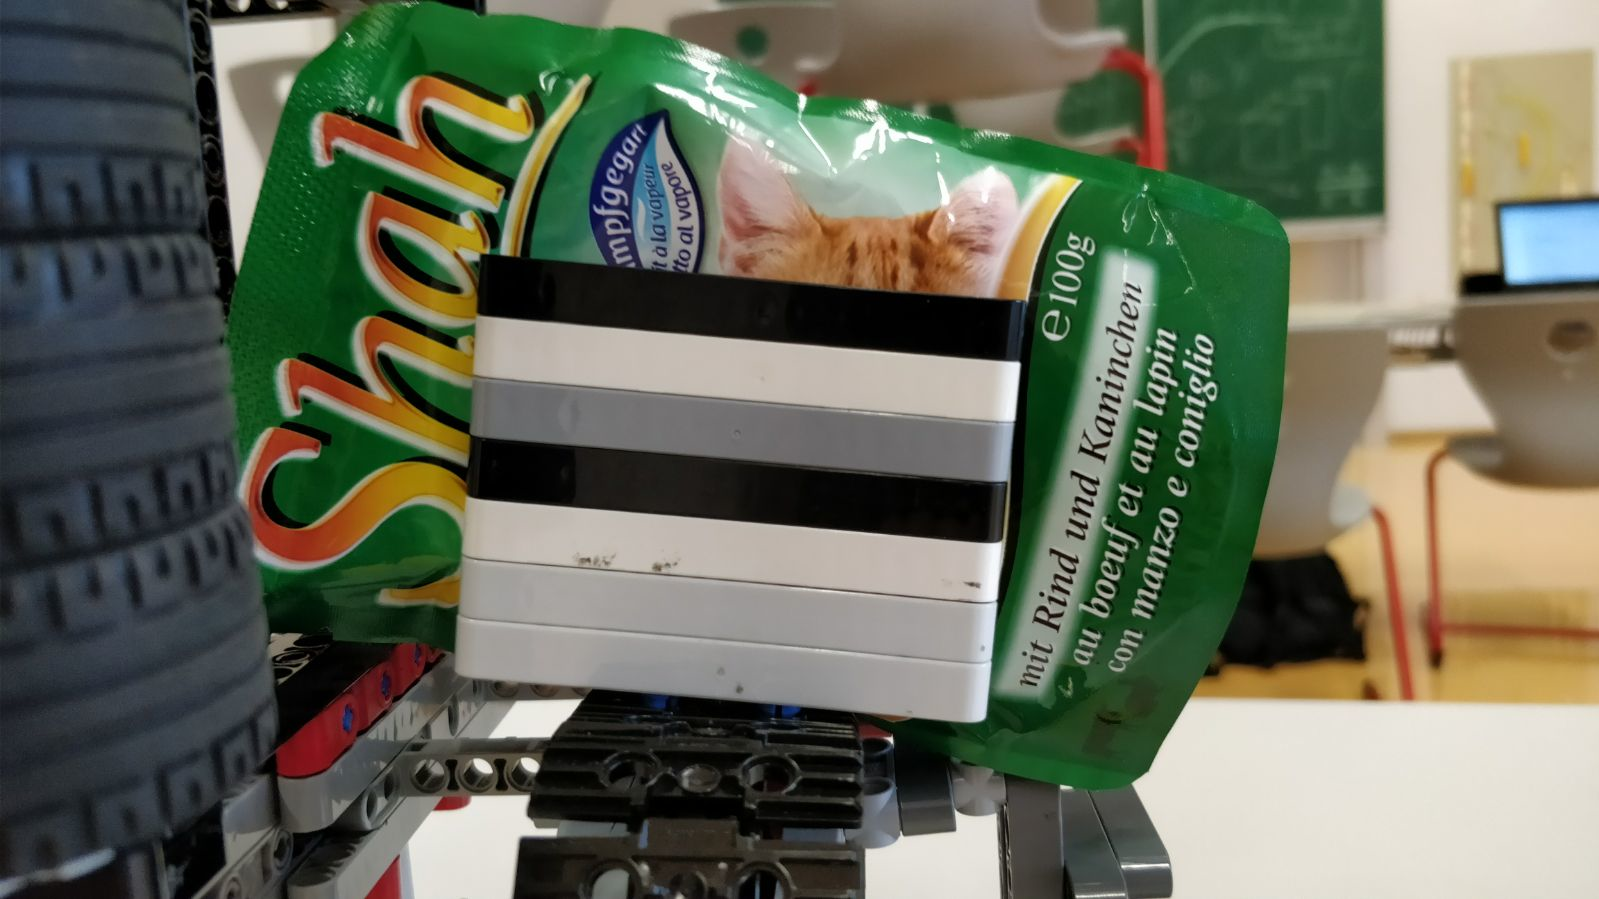
\includegraphics[width=0.50\textwidth]{Bilder/Ablauf_1_png/Magazin_Vorne}
  \end{center}
  \caption{Magazin Modellaufbau von Vorne}
  \label{Magazin Vorne}
  \vspace{-10pt}
\end{wrapfigure}

In den folgenden Bildern wird das Magazin anhand eines Aufbaues aus Lego in verschiedenen Blickwinkeln gezeigt. Hier muss man beachten das die vom Futterhersteller für die Öffnung vorgesehene Seite in Richtung des Schneidewerks zeigt (die schmale Seite mit der Einkerbung). Abbildung: \ref{Magazin Vorne}.
Das ganze Förderband besteht grundsätzlich aus der Halterung die das Magazin in einer bestimmten Höhe hält, damit die einzelnen Trennwände nicht mit dem Boden kollidieren und somit keine freie Bewegung ermöglicht ist. Der Oberteil des Bandes schließt eben mit der Schneideplattenhöhe ab um ein leichtes gleiten der Packung durch den Greifer zu ermöglichen, ohne das es Höhenunterschiede überwinden muss. Weiters wird über zwei Räder ein Band gespannt an denen die Wände in Abstand der Dicke der Packung festgemacht werden. Das Band wird mithilfe eines Motors in Bewegung gebracht und kann somit von Abteil zu Abteil bewegt werden um immer nach dem Füttern eine neue Packung bereit zu stellen. Auf diesem Band können je nach Länge eine gewissen Anzahl an Futterpackung gelegt werden, natürlich nur auf der Oberseite da die Packungen ansonsten aus den Abteilungen fallen.\\

In der Abbildung: \ref{Magazin Seitlich} wird das Magazin von der Seite gezeigt. \\
In der Abbildung: \ref{Magazin Oben} wird das Magazin von Oben gezeigt. 

\begin{figure}[H]
   \begin{minipage}[hbt]{0.5\textwidth} % [b] => Ausrichtung an \caption
      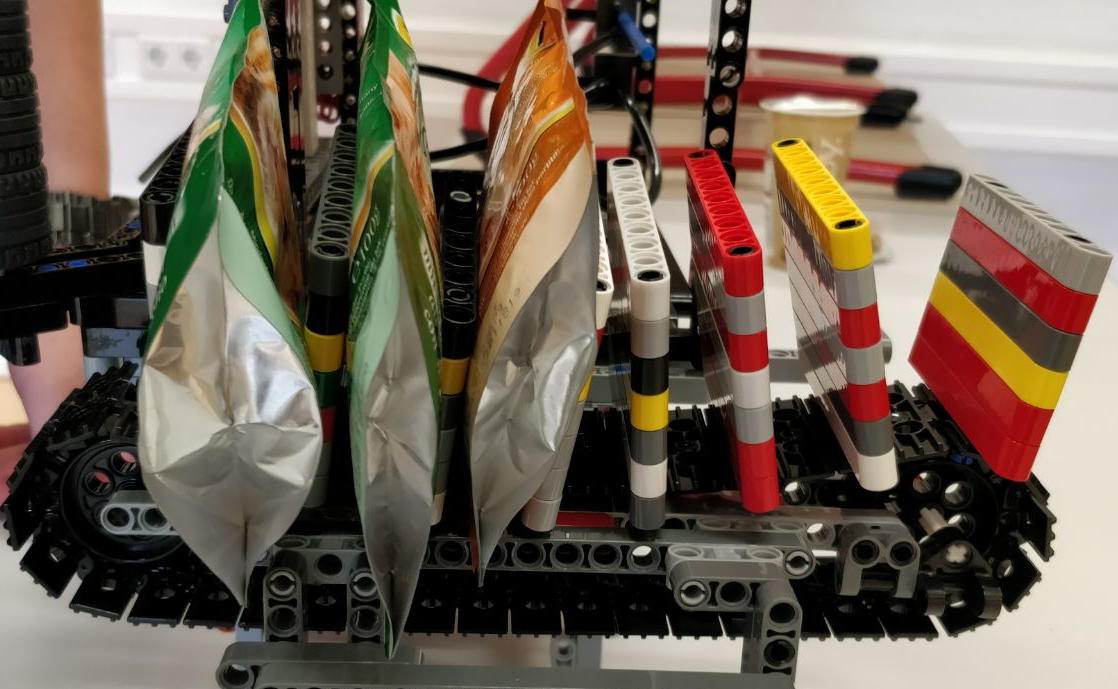
\includegraphics[width=1\textwidth]{Bilder/Ablauf_1_png/Magazin_Seitlich}
      \caption{Magazin Modellaufbau von der Seite}
      \label{Magazin Seitlich}
   \end{minipage}
   \hspace{.04\linewidth}% Abstand zwischen Bilder
   \begin{minipage}[hbt]{0.5\textwidth} % [b] => Ausrichtung an \caption
      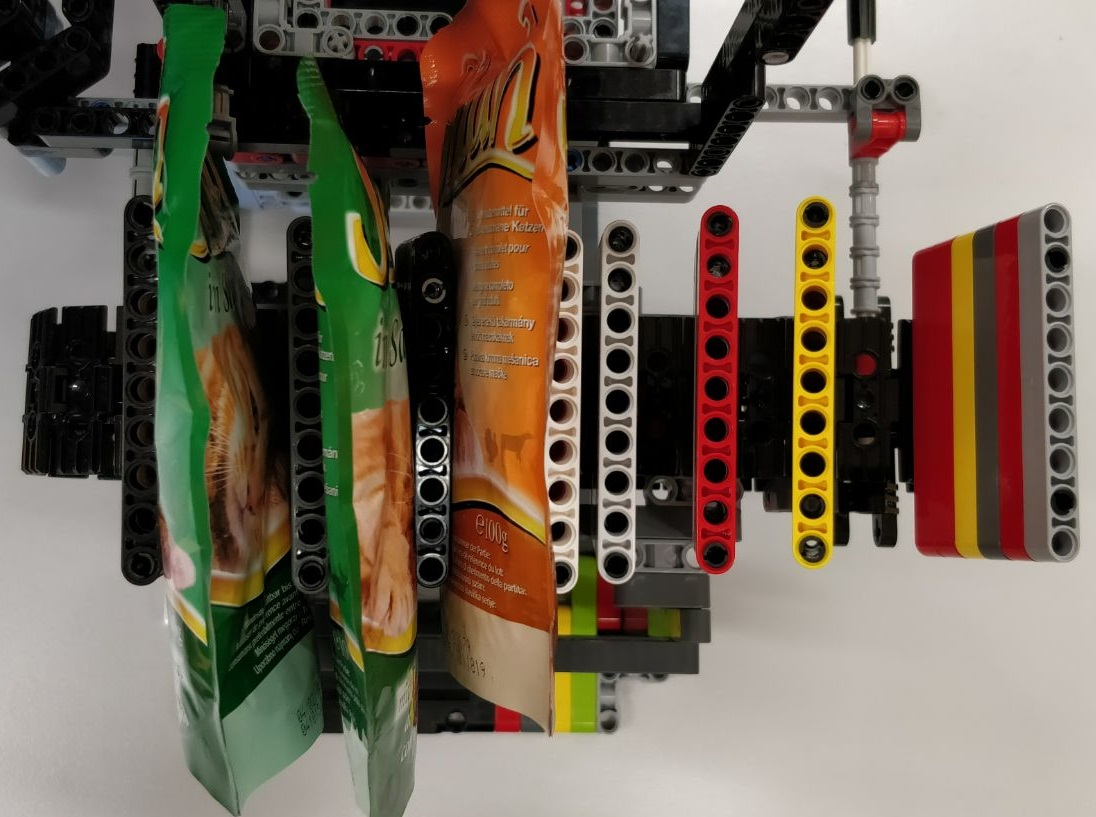
\includegraphics[width=0.92\textwidth]{Bilder/Ablauf_1_png/Magazin_Oben}
      \caption{Magazin Modellaufbau von Oben}
	  \label{Magazin Oben}      
      \end{minipage}
\end{figure}



\subsubsection{Führen zur Schneidplatte}

In diesem Schritt wird mithilfe eines Greifers (dargestellt durch eine Hand) die Packung in richtiger Position gebracht.
Durch die richtige Höhe des Förderbandes muss der Greifer keine hohe Kraft aufwenden um die Packung an ihrem Zielort zu bringen. Der Greifer dient auch noch dazu während des Schneidens neben den Magnetzylindern die Packung stabil an Stelle zu halten ohne dass der Schnittpunkt verrutscht und die Schneide nicht mehr die Einkerbung, die leichter zu Schneiden ist, trifft. Das kann zu dem Problem führen, dass man die dickere Kunstoffumhüllung schneidet und der Schnitt nicht Ordnungsgemäß durchgeführt wird. Dadurch kann der Kunstoff zwischen die Schneiden gelangen und sie damit auseinander drücken. Dadurch würde dann die Packung nicht aufgeschnitten werden können. Nur bei sehr guter Einspannung tritt beim Schnitt eine Schubbelastung auf, die einen relativ geringen Kraftaufwand für die Rissfortpflanzung erfordert. Die ertragbare Schubspannung muss immer nur punktuell in der Risskerbe überschnitten werden. Bei schlechter Einspannung besteht die Gefahr, dass die Zugspannung über einen größeren Bereich auftreten würde, was enorme Kräfte erfordern würde. Siehe Abbildungen: \ref{Magazin Auszug}, \ref{Magazin Mitte}

\begin{figure}[H]
   \begin{minipage}[hbt]{0.5\textwidth} % [b] => Ausrichtung an \caption
      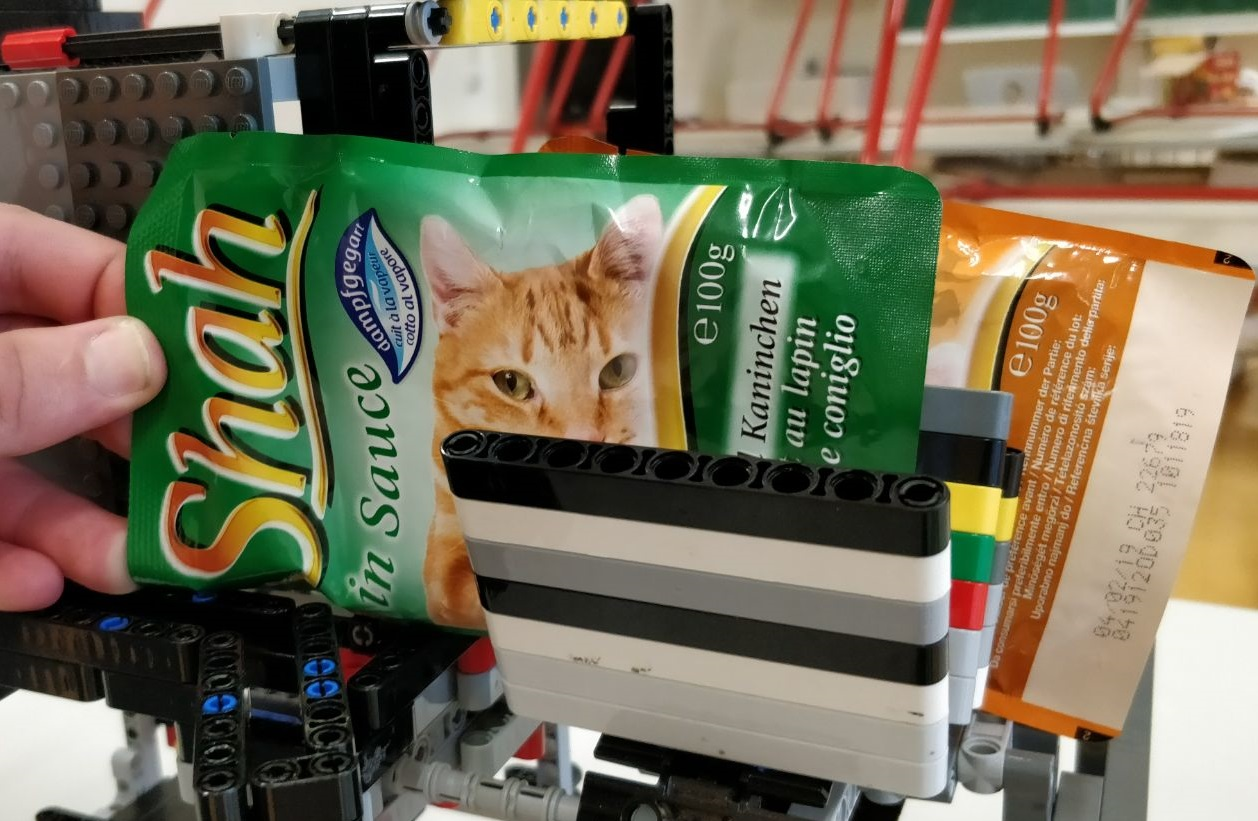
\includegraphics[width=1\textwidth]{Bilder/Ablauf_1_png/Magazin_Auszug}
      \caption{Magazin Auszug}
      \label{Magazin Auszug}
   \end{minipage}
   \hspace{.04\linewidth}% Abstand zwischen Bilder
   \begin{minipage}[hbt]{0.5\textwidth} % [b] => Ausrichtung an \caption
      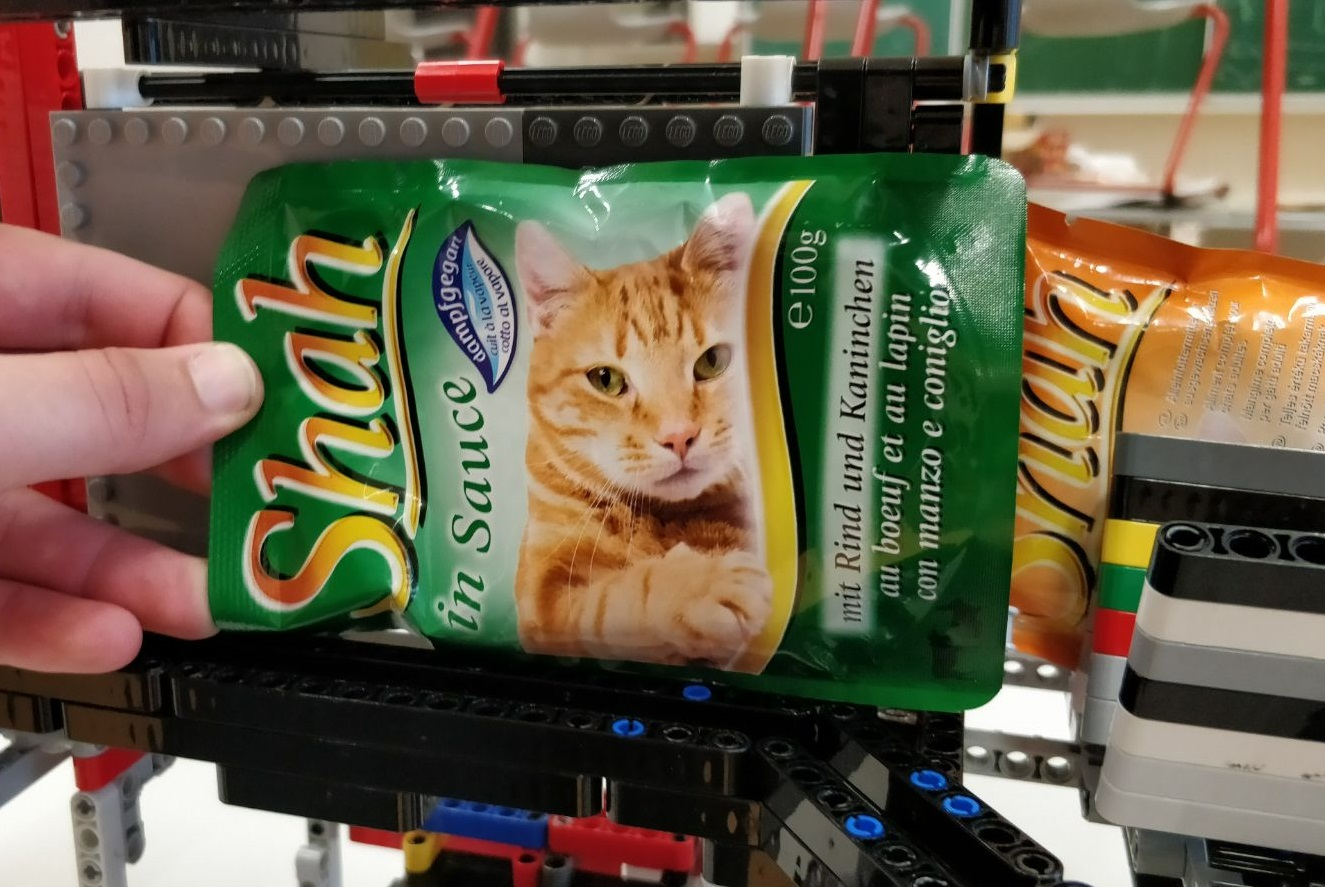
\includegraphics[width=0.92\textwidth]{Bilder/Ablauf_1_png/Magazin_Auszug_2}
      \caption{Magazin Auszug Mitte}
	  \label{Magazin Mitte}      
      \end{minipage}
\end{figure}

\vspace{20pt}

\begin{wrapfigure}{r}{0.5\textwidth}
\vspace{-30pt}
  \begin{center}
    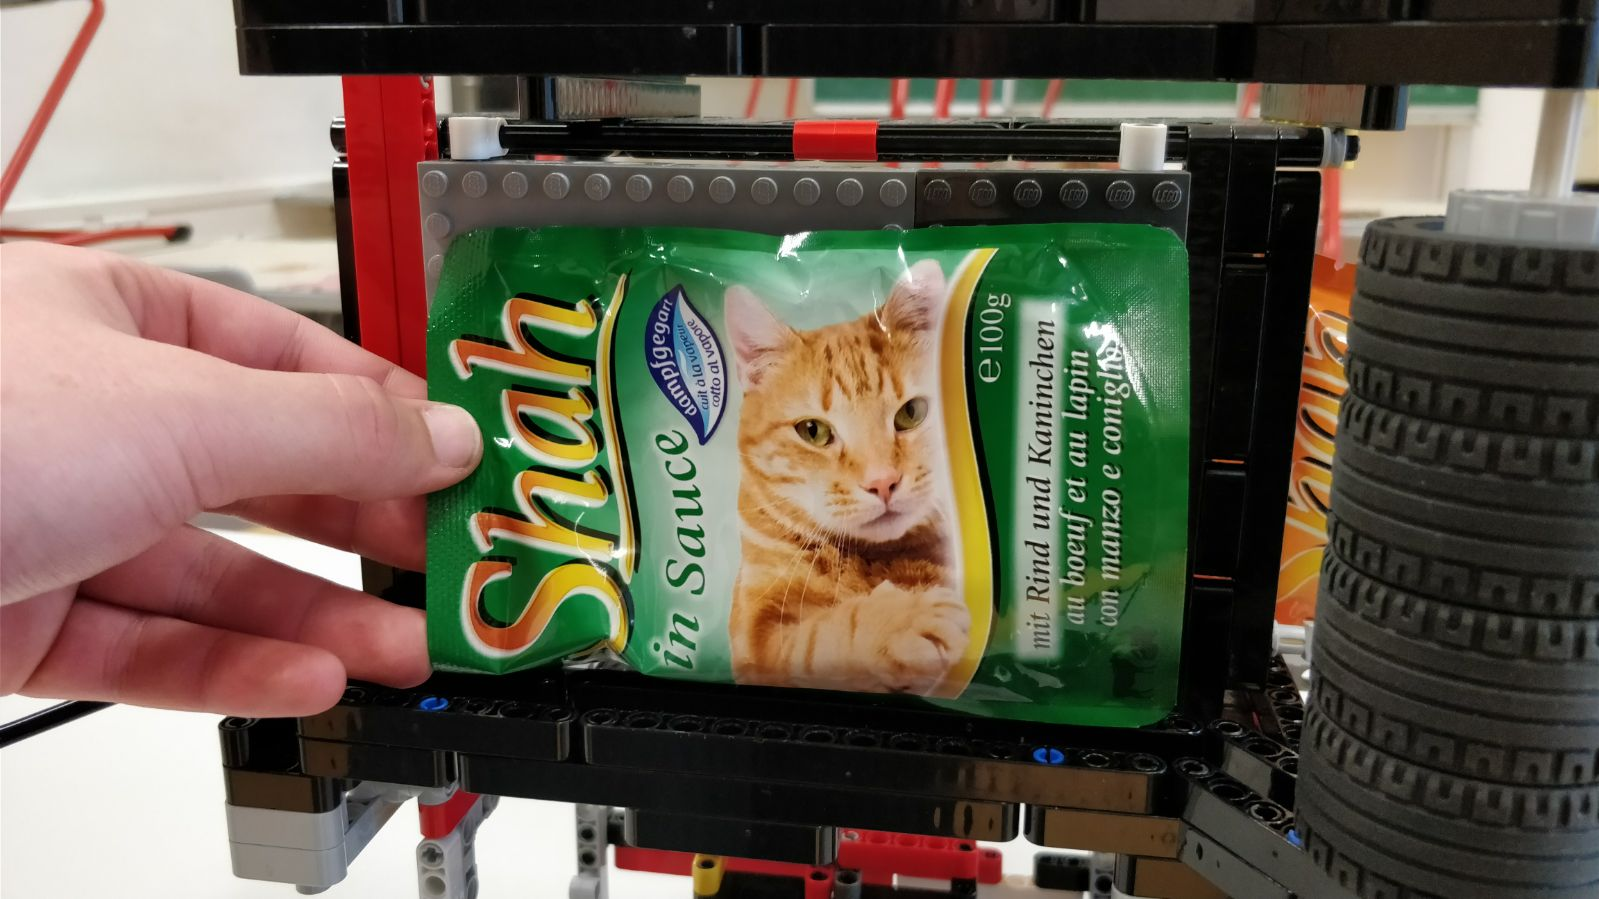
\includegraphics[width=0.50\textwidth]{Bilder/Ablauf_1_png/Schneidebereit}
  \end{center}
  \caption{Schneidebereit}
  \label{Schneidebereit}
  \vspace{-10pt}
\end{wrapfigure}

Wie im Bild \ref{Schneidebereit} gezeigt liegt das Katzenfutterpackerl in der richtigen Position und wird mit zwei Magnetzylindern an der Schneidefläche festgehalten. Die Magnetzylinder haben genügend Kraft um die Packung auch während des Schnittes und der Walzphase in Position zu halten. Wenn die Packung verrutschen würde könnte im schlimmsten Fall die Funktion der Maschine beeinflusst werden, indem sie den Greifer oder das Förderband blockiert. Daraufhin müsste die Maschine manuell geöffnet und der Beutel per Hand raus geholt werden. \newpage
\subsubsection{Schnitt}

\begin{wrapfigure}{r}{0.5\textwidth}
\vspace{-30pt}
  \begin{center}
    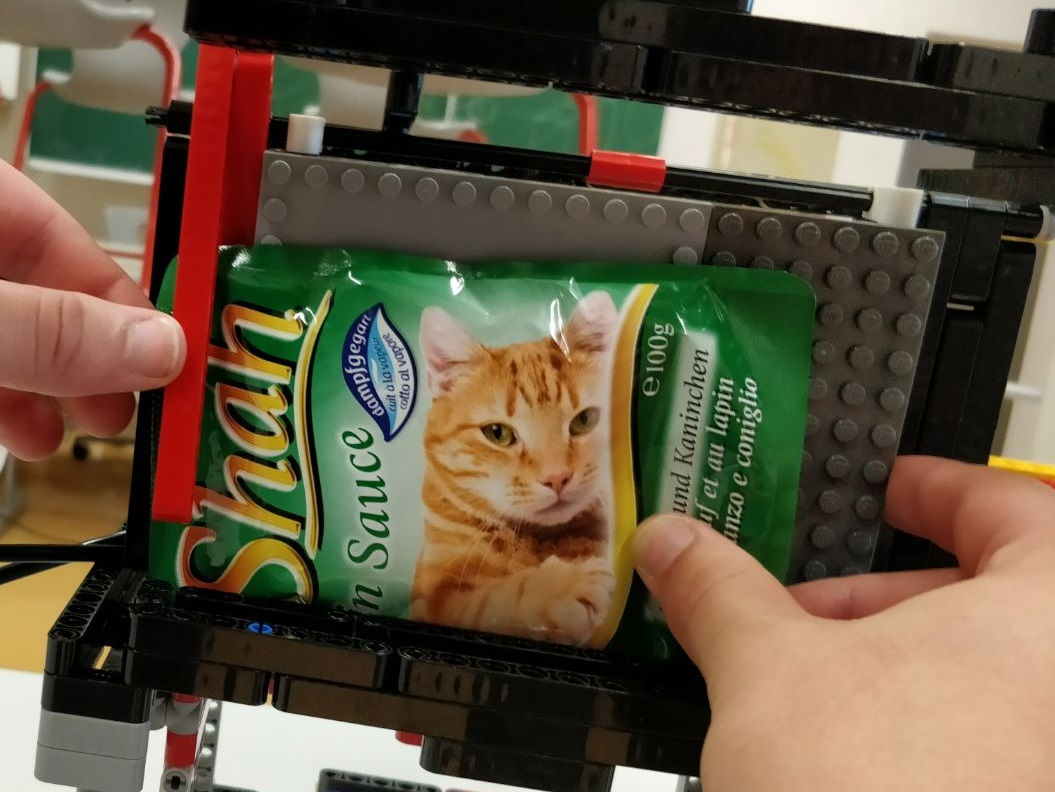
\includegraphics[width=0.50\textwidth]{Bilder/Ablauf_1_png/Schnitt}
  \end{center}
  \caption{Schnitt}
  \label{Schnitt}
  \vspace{-10pt}
\end{wrapfigure}

In der richtigen Position muss man mit 2 scharfen Klingen mit viel Kraft die Packung aufschneiden. Eine davon wird an der Schnittfläche angebracht und die andere macht die Schneidbewegung, wobei die beiden aneinander reibenden Kanten den Schnitt verursachen. Die Packung kann mit einem Schnitt vollständig geöffnet werden. Mit zu wenig Druck gelangt zu viel Kunstoffmaterial zwischen die Schneideflächen und durch die Länge der Schneiden biegen sie sich auseinander und somit kommt kein ordentlicher Schnitt zusammen (Zugspannung statt örtliche Schubspannung). Bei öfteren Auftritts dieses besprochenen Problems bei der selben Packung kann es zufolge haben, dass sich die Packung nicht mehr mit der Maschine schneiden lässt, weil sie sich durch die vielen Versuche verformt hat. Siehe Abbildung: \ref{Schnitt} \\

Eine andere Alternative wäre ein feingezähntes Schneiderad mit hoher Drehzahl. Versuche mit einem gezähnten Messer haben gezeigt etwa 9 Schnitte mit einem Messer erforderlich waren um eine 10cm Verpackung vollständig aufzuschneiden.


\subsubsection{Pressen}

\begin{wrapfigure}{r}{0.5\textwidth}
\vspace{-30pt}
  \begin{center}
    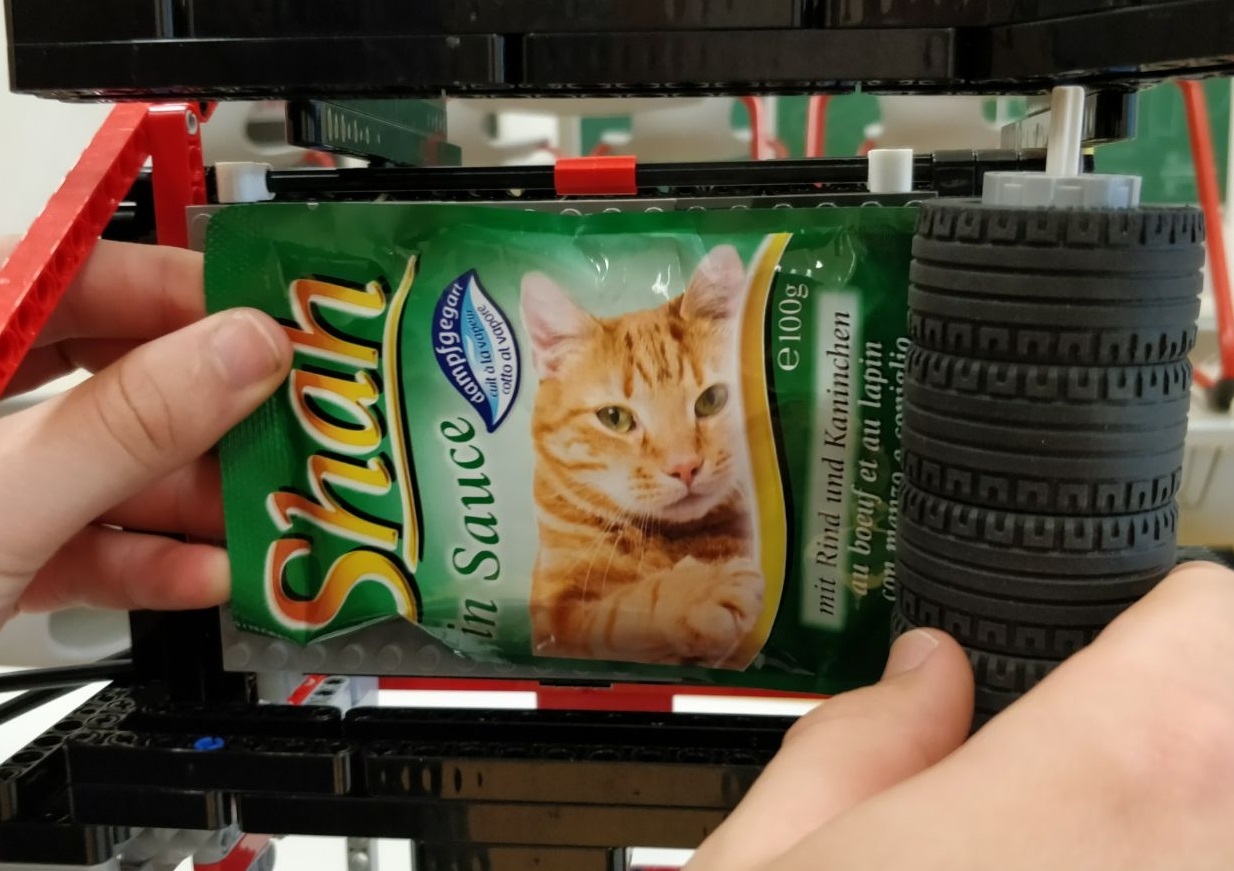
\includegraphics[width=0.50\textwidth]{Bilder/Ablauf_1_png/Ausquetschen_1}
  \end{center}
  \caption{Ausquetschen Beginn}
  \label{Ausquetschen Beginn}
  \vspace{-10pt}
\end{wrapfigure}

Nach dem Aufschneiden wird mit einer Rolle die Packung ausgepresst. Dazu werden zuerst die ersten 2 Magnetzylinder gelöst bis die Rolle vorbei ist. Danach werden sie wieder in Position gebracht. Daraufhin werden die anderen beiden gelöst und die Rolle fährt ans Ende. Die Rolle ist auf einer Welle platziert, diese wird mit 2 Sicherungsringen an einer  vorgegebenen Position befestigt. Die Rolle ist 10 cm breit, damit ohne Probleme die 9,4cm breite Futterpackung ausgepresst werden kann. Sie wird in einer Vorrichtung an der Maschine angehängt und steht mit einem bestimmten Winkel auf die Schneidfläche damit ein großer Anpressdruck entsteht. Durch die schmierige Konsistenz gleitet das Futter aus der Verpackung und wird nicht von der Walze zerquetscht. Nach der Beseitigung der Verpackung werden zuerst die beiden Magnetzylinder von der Maschine entfernt in Anfangsposition gebracht, damit die Walze ohne Probleme in Startposition zurückkehren kann. Siehe Abbildungen: \ref{Ausquetschen Beginn}, \ref{Ausquetschen Mitte}, \ref{Ausquetschen Ende}



\begin{figure}[H]
   \begin{minipage}[hbt]{0.5\textwidth} % [b] => Ausrichtung an \caption
      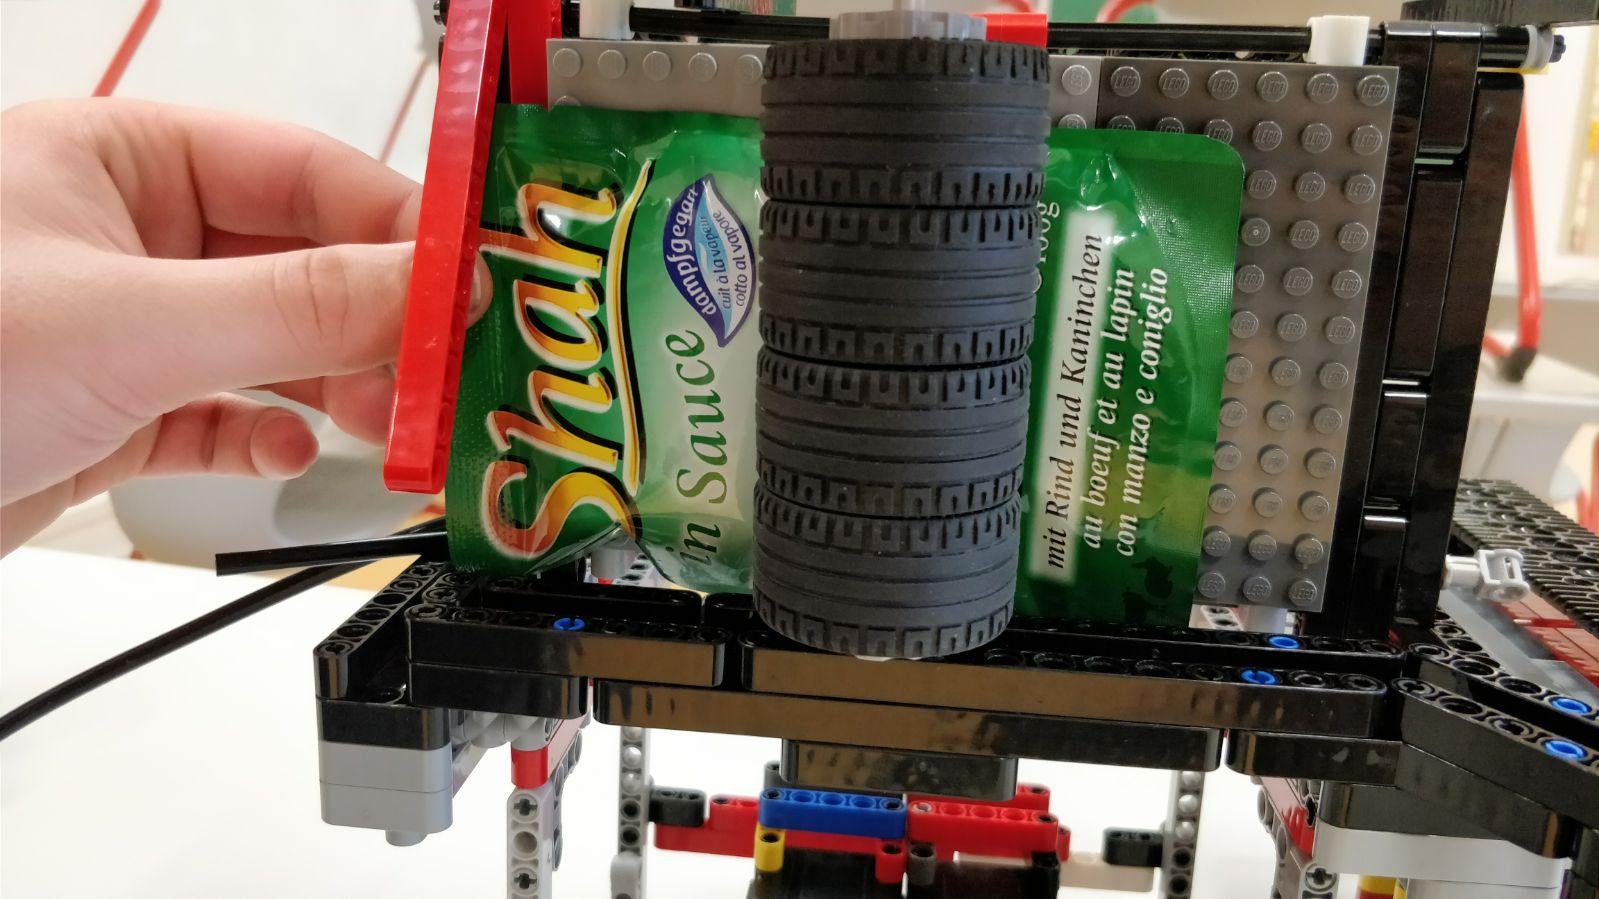
\includegraphics[width=1\textwidth]{Bilder/Ablauf_1_png/Ausquetschen_2}
      \caption{Ausquetschen Mitte}
      \label{Ausquetschen Mitte}
   \end{minipage}
   \hspace{.04\linewidth}% Abstand zwischen Bilder
   \begin{minipage}[hbt]{0.5\textwidth} % [b] => Ausrichtung an \caption
      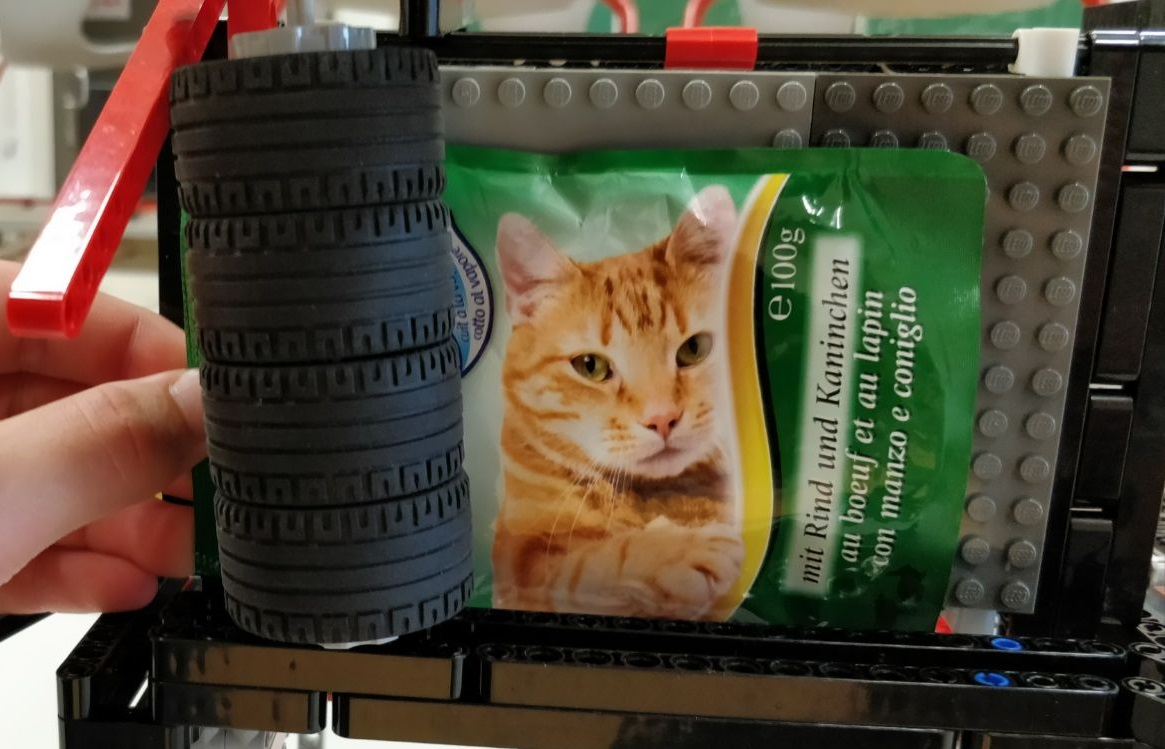
\includegraphics[width=0.98\textwidth]{Bilder/Ablauf_1_png/Ausquetschen_3}
      \caption{Ausquetschen Ende}
	  \label{Ausquetschen Ende}      
      \end{minipage}
\end{figure}

Eine andere Alternative wäre ein senkrechtes Ausquetschen nach unten, unterstützt von der Schwerkraft. Dies ist bei dieser Variante schwer zu realisieren.

\subsubsection{Entsorgen}

\begin{wrapfigure}{r}{0.5\textwidth}
\vspace{-30pt}
  \begin{center}
    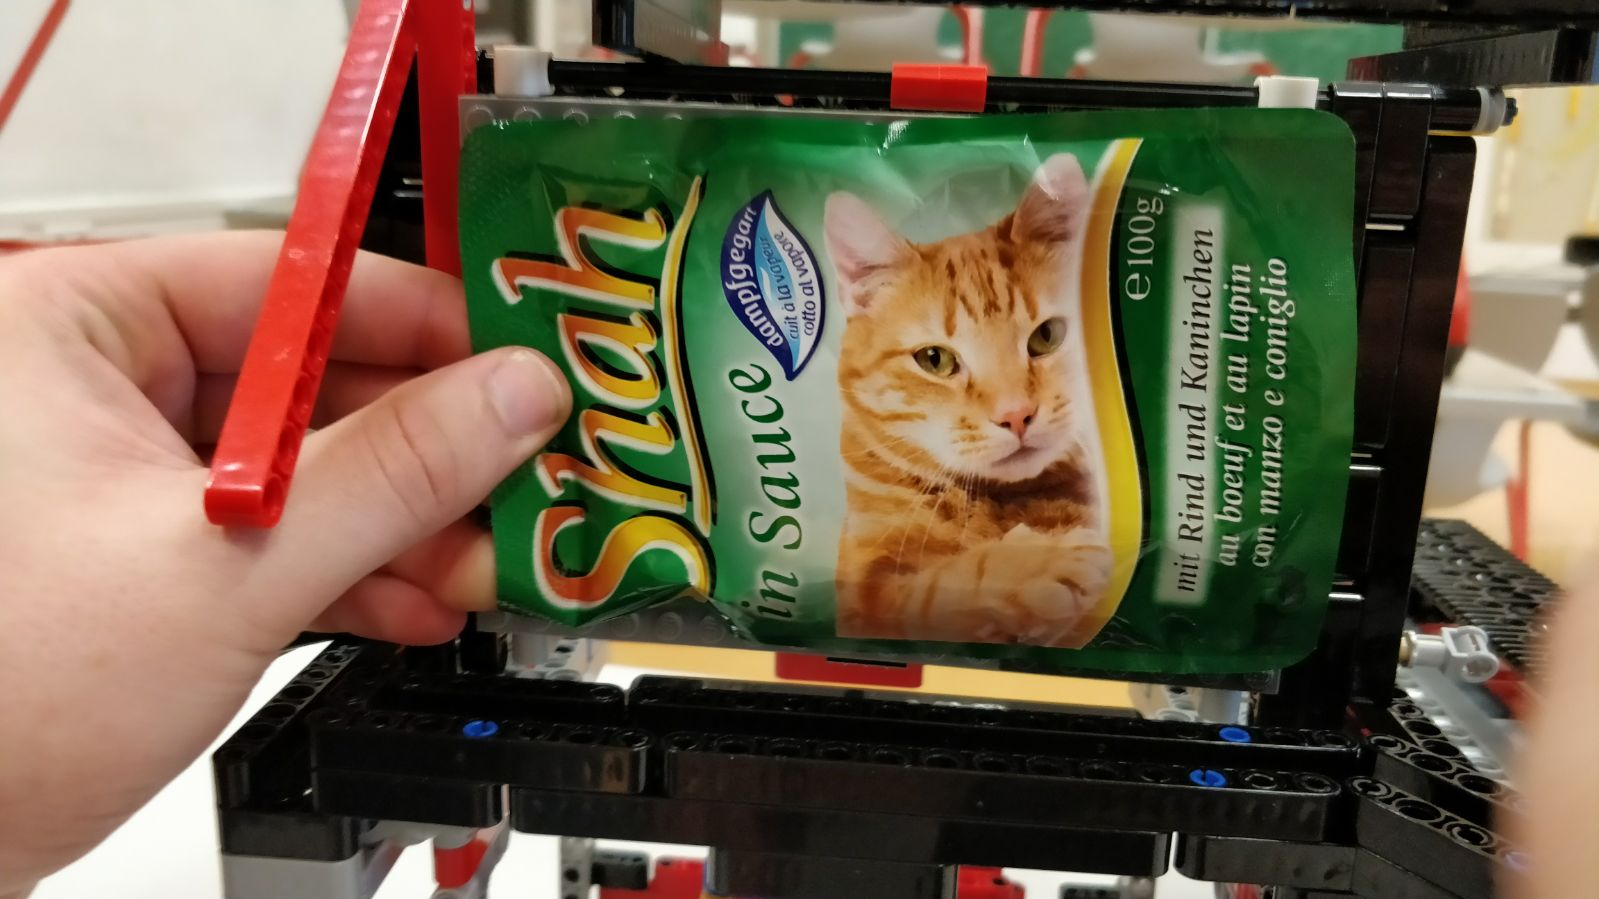
\includegraphics[width=0.50\textwidth]{Bilder/Ablauf_1_png/Auswurf_1}
  \end{center}
  \caption{Auswurf Beginn}
  \label{Auswurf Beginn}
  \vspace{-10pt}
\end{wrapfigure}

Nach dem Auspressen wird die leere Packung durch die Rückklappe in einen Luftdichten Container geworfen. Die Klappe wird durch zwei Stifte gehalten und lässt sich durch ein Scharnier nach hinten klappen. Die zwei Stifte sind mit Kosten verbunden da 2 Magnetzylinder benötigt werden und die in einem Schaltplan zu berücksichtigt sind. Außerdem benötigen sie zusätzlich Platz. Die Klappe befindet sich hinter der Futterverpackung. Siehe Abbildung: \ref{Auswurf Beginn}. \\

In der Abbildung: \ref{Bolzen drinnen} sieht man den Stift (Oranger Kreis) der ein vorzeitiges nach Hinten klappen verhindert. Die Stifte müssen so dimensioniert sein damit sie die Kräfte der Walze aushält. \\

In der Abbildung: \ref{Bolzen entfernen} wurde der Bolzen entfernt (Oranger Kreis) und somit lässt sich die Klappe nach hinten klappen. 

\begin{figure}[H]
   \begin{minipage}[hbt]{0.5\textwidth} % [b] => Ausrichtung an \caption
      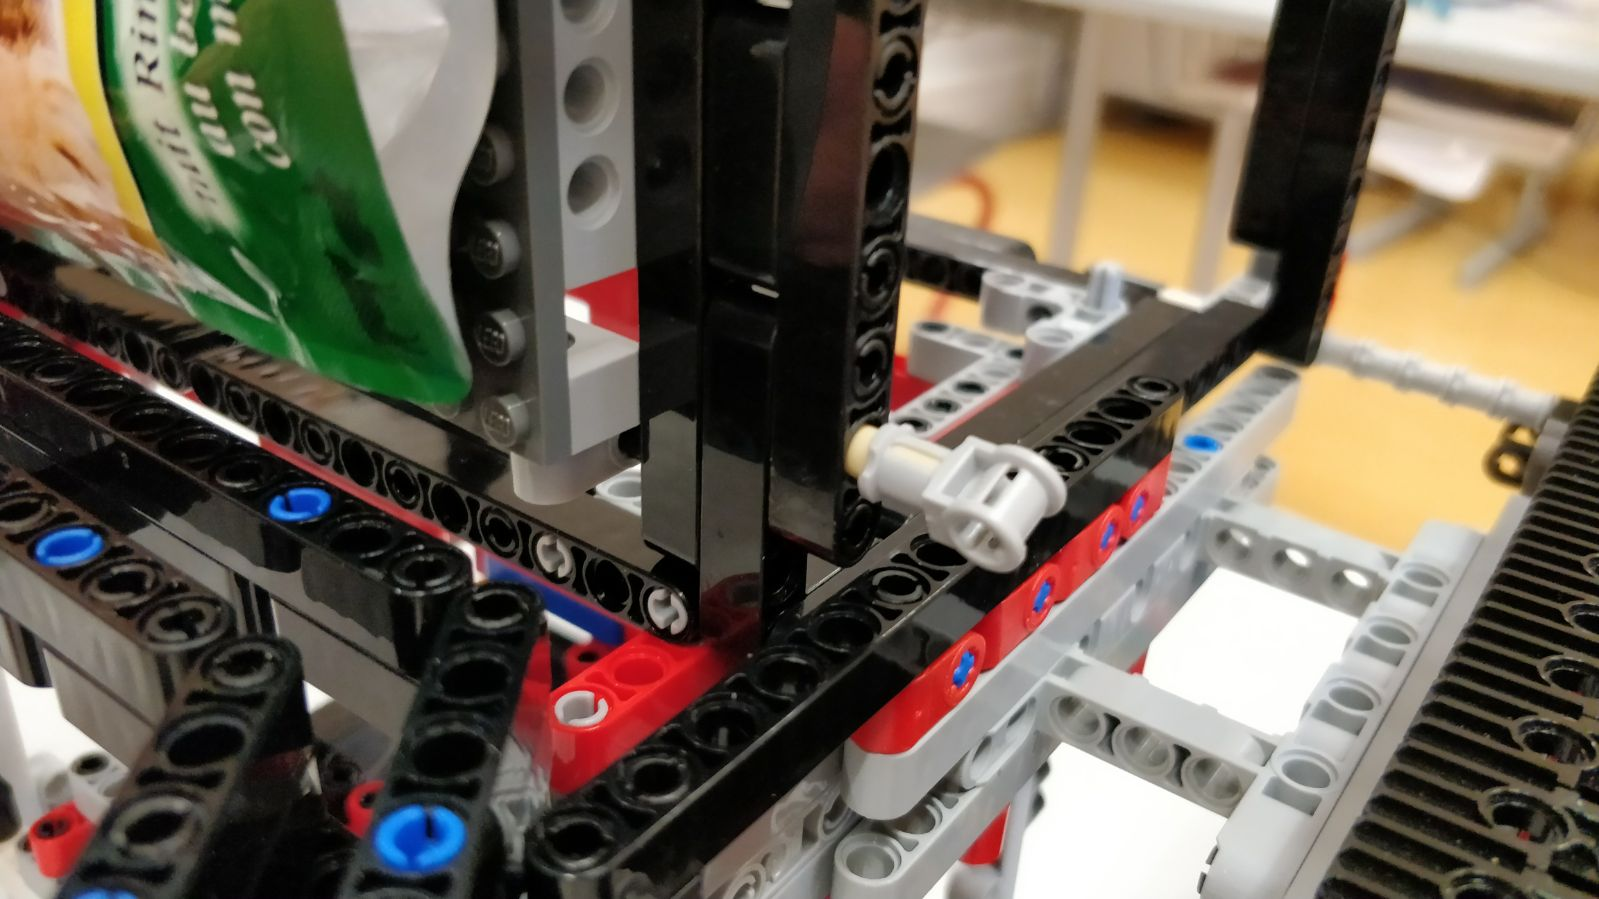
\includegraphics[width=1\textwidth]{Bilder/Ablauf_1_png/Auswurf_2}
      \caption{Bolzen drinnen}
      \label{Bolzen drinnen}
   \end{minipage}
   \hspace{.04\linewidth}% Abstand zwischen Bilder
   \begin{minipage}[hbt]{0.5\textwidth} % [b] => Ausrichtung an \caption
      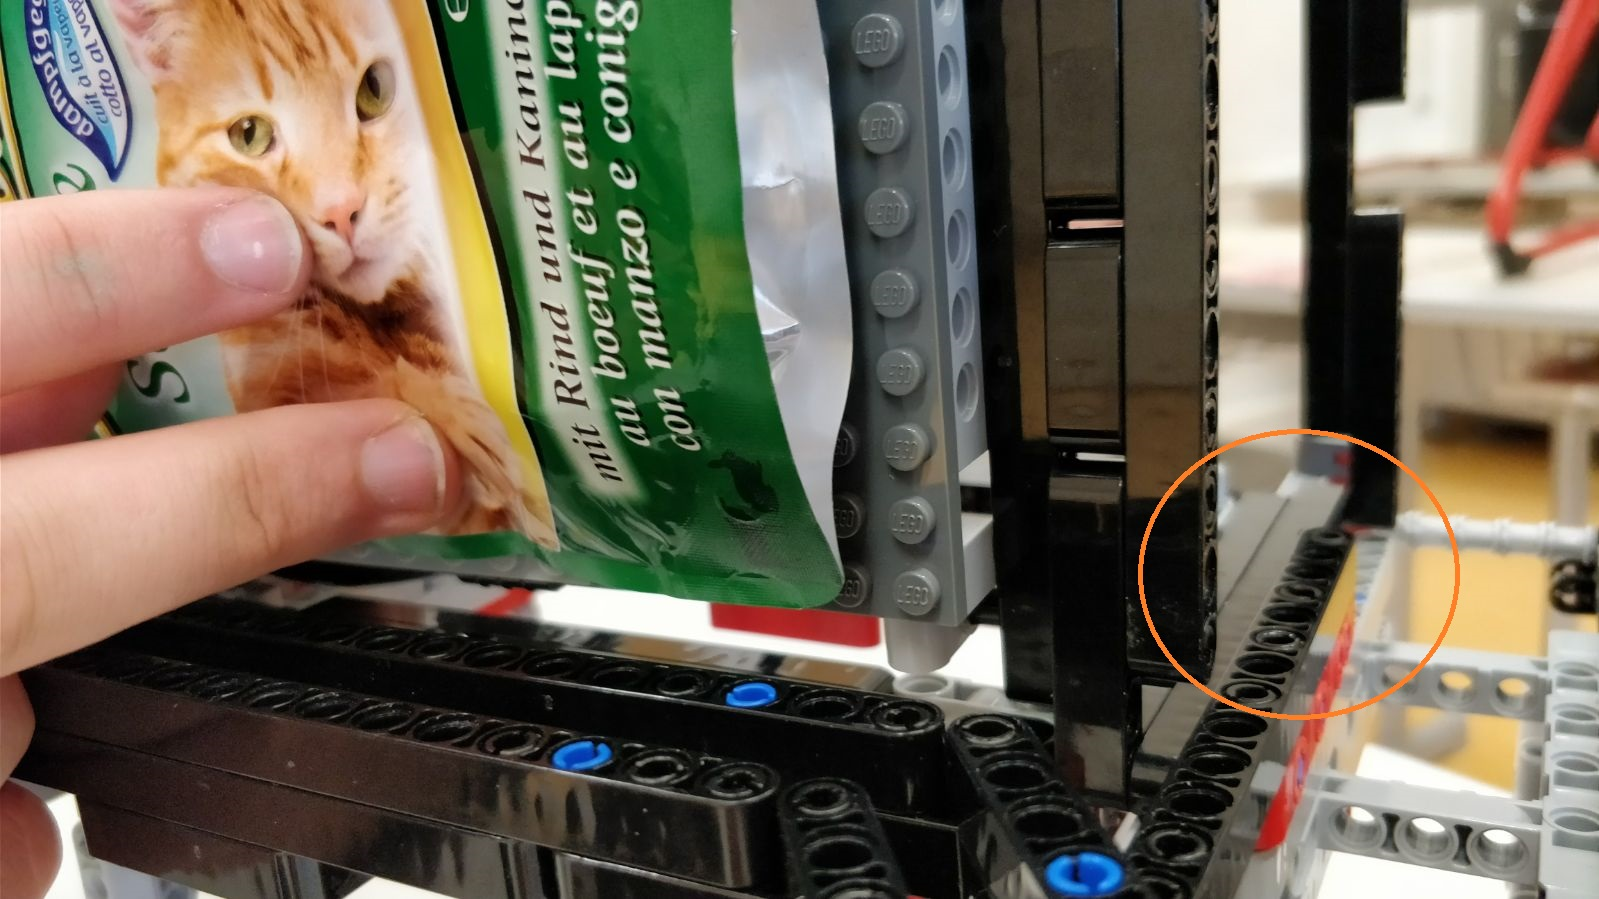
\includegraphics[width=1\textwidth]{Bilder/Ablauf_1_png/Auswurf_3}
      \caption{Bolzen entfernen}
	  \label{Bolzen entfernen}      
      \end{minipage}
\end{figure}


In der Abbildung: \ref{Klappe öffnen} wird demonstriert wie die Magnetzylinder die leere Packung gegen die Klappe drücken, wodurch die Klappe sich öffnet und die leere Packung hinunterfällt.\\

In der Abbildung: \ref{Fertiger Auswurf} sieht man sehr gut wie die Klappe aussieht und wie sie nach hinten aufgeht und der Futtersack in der luftdichten Box entsorgt wird.


\begin{figure}[H]
   \begin{minipage}[hbt]{0.5\textwidth} % [b] => Ausrichtung an \caption
      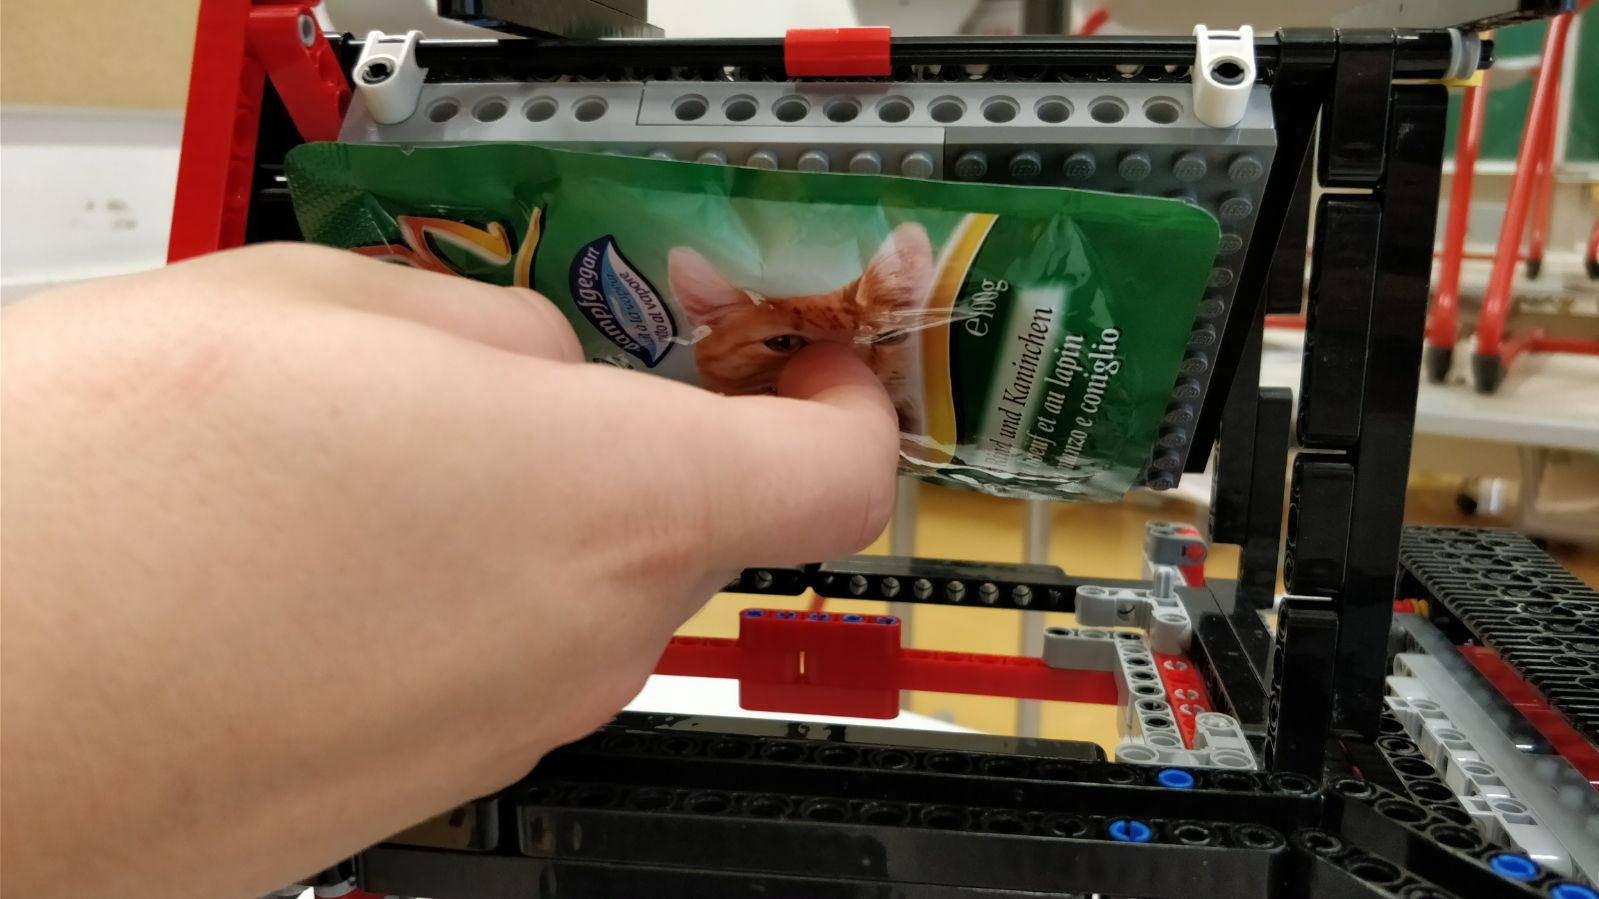
\includegraphics[width=1\textwidth]{Bilder/Ablauf_1_png/Auswurf_4}
      \caption{Klappe öffnen}
      \label{Klappe öffnen}
   \end{minipage}
   \hspace{.04\linewidth}% Abstand zwischen Bilder
   \begin{minipage}[hbt]{0.5\textwidth} % [b] => Ausrichtung an \caption
      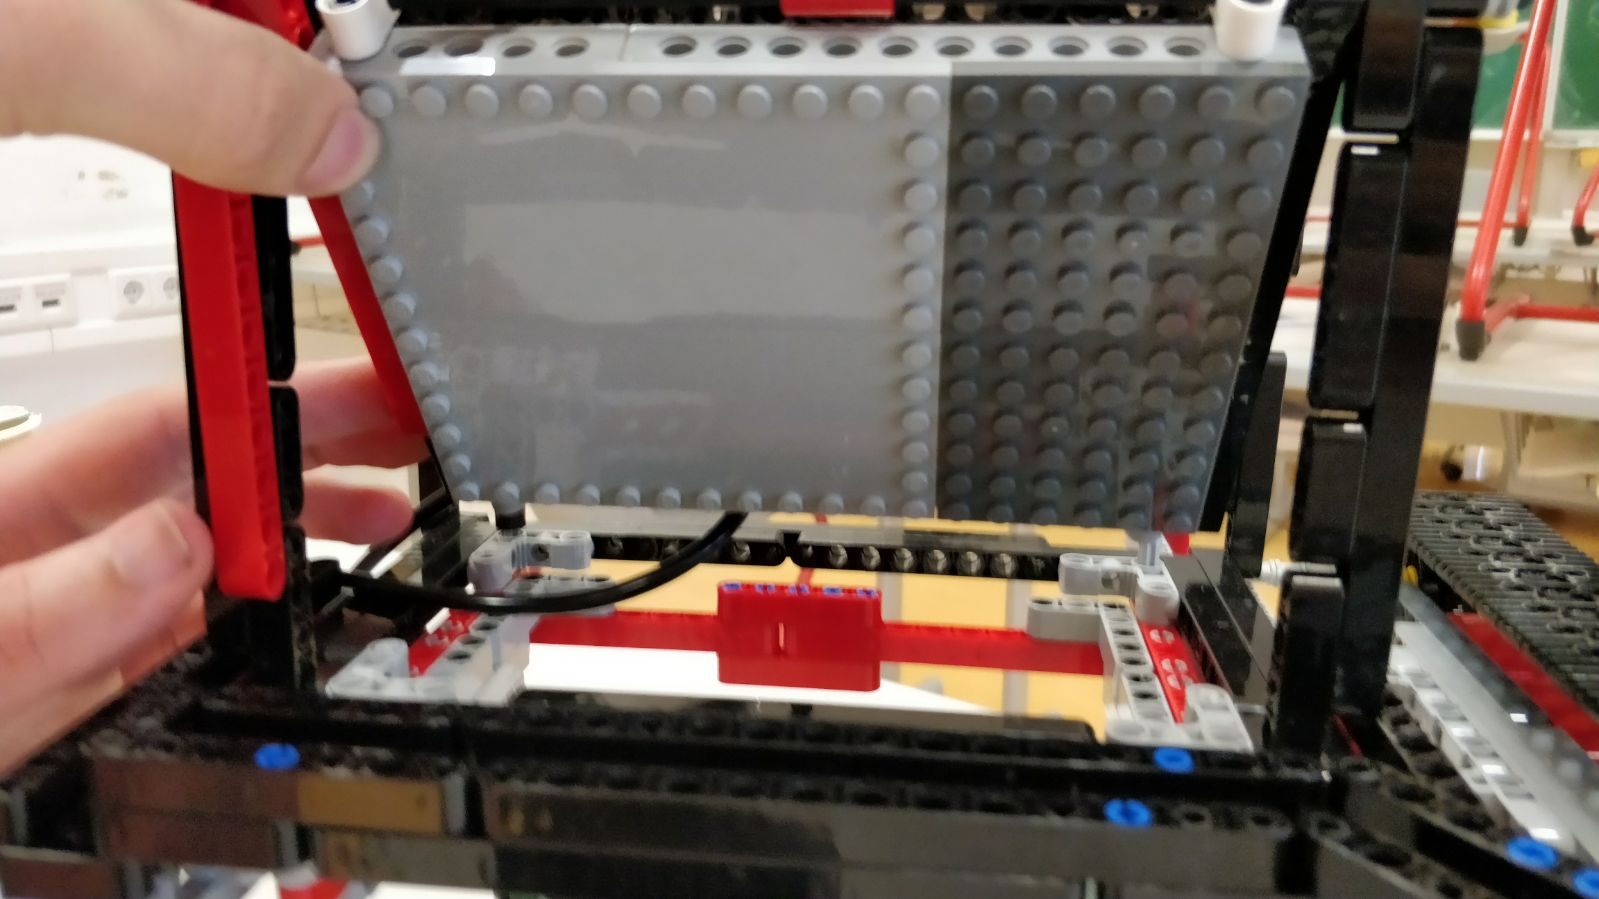
\includegraphics[width=1\textwidth]{Bilder/Ablauf_1_png/Auswurf_5}
      \caption{Fertiger Auswurf}
	  \label{Fertiger Auswurf}      
      \end{minipage}
\end{figure}


\subsubsection{Füttern}

\begin{wrapfigure}{r}{0.5\textwidth}
\vspace{-40pt}
  \begin{center}
    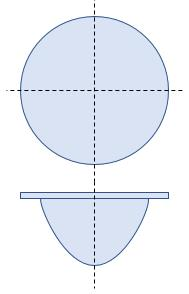
\includegraphics[width=0.17\textwidth]{Bilder/Powerpoint/Loch_Futterschuessel}
  \end{center}
  \caption{Loch Futterschüssel}
  \label{Loch_Futterschuessel}
  \vspace{-10pt}
\end{wrapfigure}

Die Maschine besitzt 5 Futterschüsseln die auf einer drehbaren Platte stehen. Vor dem Füttern wird eine saubere Platte unter der Stelle, wo später die Packung aufgeschnitten wird, positioniert. Während es ausgepresst wird, fällt das Futter in die Futterschüssel. Wenn der Auspressvorgang beendet ist, wird die Futterschüssel an eine Position bewegt, wo die Katze Zugang zum fressen hat. Die Schüsseln lassen sich einfach aus der Halterung nehmen da sie nur in einem Loch in der Platte liegen. Das hat den Vorteil gegenüber anderen Schüsseln die auf der Platte montiert sind, dass die Katze nicht soweit zur Futterschüssel hat d.h. sie muss nur mit dem Kopf zur Plattenoberfläche und nicht Platte + Schlüsselhöhe, somit spart man je nach Schüssel wertvolle Zentimeter. Die Platte ist mit einer Gummischicht überzogen damit die Schüssel, durch der Kopf der Katze, wenn sie frisst, nicht verrutsch. Sie lässt sich aus der Platte entnehmen, indem der Benutzer mit der Hand die Futterschüssel von unten durch das loch drückt und mit der anderen Hand entnimmt. Danach werden die Schüsseln gewaschen, getrocknet und die Schüssel in das Loch fallen gelassen. Siehe Abbildung: \ref{Loch_Futterschuessel}



\subsection{Variante 2: Vor aufgeschnittene Packung }

Diese Variante wurde entwickelt um den Schneidemechanismus zu umgehen, da dieser keine leichte Unterfangen ist. Hierbei wird jedoch der Benutzer aufgefordert mehr Zeit in die Maschine zu investieren als bei den anderen Varianten. Er muss sämtliche Packungen aufschneiden mit einer Klemme versehen und in das Förderband einhängen. Mit dieser Bauweise wird viel auf die Hilfe der physikalischen Kräfte gesetzt. Zum Großteil funktioniert das Prinzip mit der Schwerkraft der die Packung entleeren soll.

\subsubsection{Förderband und Kettenglieder}

Beim Förderband erkennt man wo sich die Futterpackungen befinden sollen. Es wird über die zwei Kettenräder eine Kette gespannt. Auf diese Kette werden die Futterpackungen gehängt, dass funktioniert aber nur weil die Kettenglieder einen rechen Winkel auf jeder Seite hat (siehe Abbildung: \ref{Kettenglied}). Auf diesen Winkel wird eine Aluplatte geschraubt und mit einer anderen Platte festgeklemmt. Die Kette wird mithilfe eines Kettenrades und eines Motors in Bewegung gebracht, damit bewegt sich die Packung immer näher Richtung Walze. Dadurch die Packung senkrecht auf das Förderband gehängt wird, spielt die Schwerkraft eine große Rolle und unterstützt den Entleerungsprozess der Katzenfutterpackung.\\ Die zwei dunkelblauen Kreise symbolisieren die zwei Kettenräder die die Kette antreiben. Um die Kreise liegen die einzelnen Kettenglieder, verbunden zu einer Kette. Die Pfeile sollen die Futterpackungen darstellen die am Schaft an der Kette befestigt sind und mit der Öffnung(Pfeilspitzen) nach unten zeigen. Siehe Abbildung: \ref{Foerderband}. \\
Die dunklere von den blauen Flächen ist die die Oberseite des rechten Winkels mit zwei Löchern zur Befestigung der Aluplatte. Die hellere Fläche ist die Unterseite des Winkels. Die Bolzen des Kettengliedes sind Orange eingezeichnet. Siehe Abbildung: \ref{Kettenglied}.

\begin{figure}[H]
   \begin{minipage}[hbt]{.3\linewidth} % [b] => Ausrichtung an \caption
      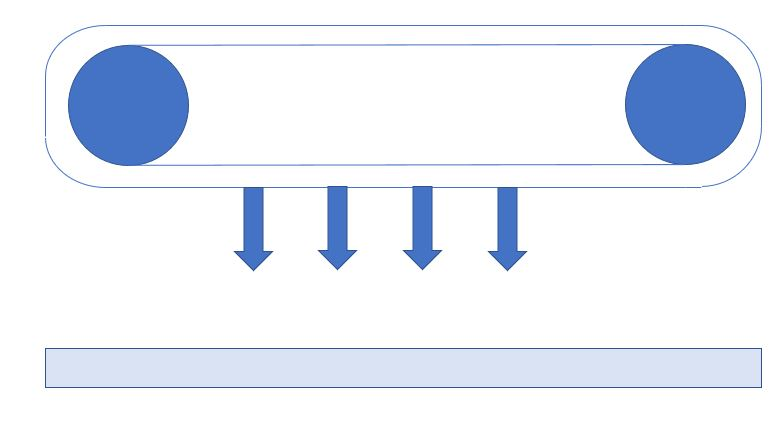
\includegraphics[width=\linewidth]{Bilder/Powerpoint/Foerderband}
      \caption{Foerderband}
      \label{Foerderband}
   \end{minipage}
   \hspace{.3\linewidth}% Abstand zwischen Bilder
   \begin{minipage}[hbt]{.3\linewidth} % [b] => Ausrichtung an \caption
      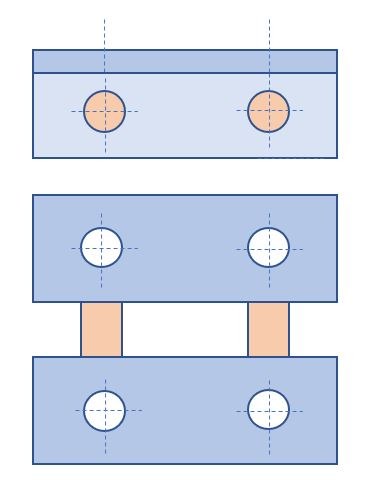
\includegraphics[width=\linewidth]{Bilder/Powerpoint/Kettenglied}
      \caption{Kettenglied}
	  \label{Kettenglied}      
      \end{minipage}
\end{figure}

\subsubsection{Walze}

Nach dem die Futterpackung in Bewegung ist, wird bei einer gewissen Position die Klemme entfernt und durch die Walze gepresst. Die Walze ist innen hohl und wird auf der Welle platziert. Die erste Walze auf der Antriebsseite und die zweite Welle auf einer eigen gefertigten Welle. Beide Walzen werden durch eine Feder aneinander gepresst, nur so stark, damit die Halterung, an der die Packung festgemacht ist, durchkommt. Dennoch so stark damit sich die Packung entleert. Die Walze an der eigen gefertigten Welle wird mit zwei Aluplatten und einem Scharnier in Stellung gehalten.\\ 
Auf der Walze ist ein Pfeil gezeichnet, der Pfeil stellt eine Futterpackung da und die Pfeilrichtung zeigt die Richtung in der die Packung ausgepresst wird. Siehe Abbildungen: \ref{Walze}. \\
Das dunkelblaue ist das eigentliche Scharnier, die hellblauen Flächen sind die Verlängerungen. Siehe Abbildungen: \ref{Scharnier}.

\begin{figure}[H]
   \begin{minipage}[hbt]{.4\linewidth} % [b] => Ausrichtung an \caption
      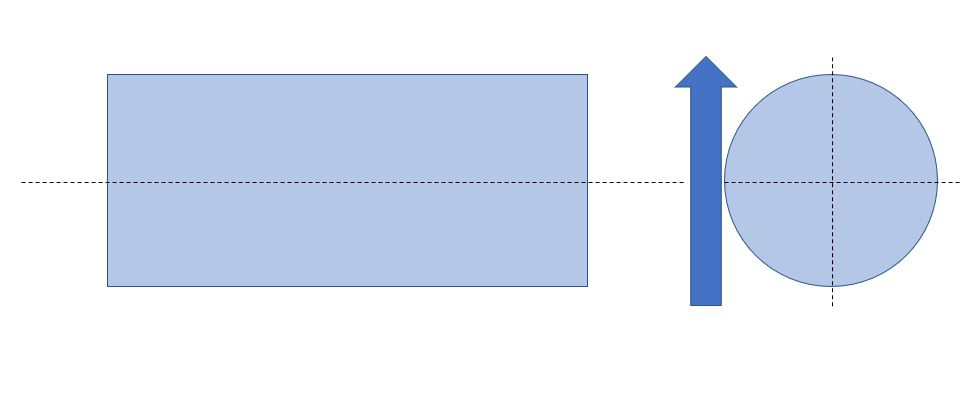
\includegraphics[width=\linewidth]{Bilder/Powerpoint/Walze}
      \caption{Walze}
      \label{Walze}
   \end{minipage}
   \hspace{.2\linewidth}% Abstand zwischen Bilder
   \begin{minipage}[hbt]{.4\linewidth} % [b] => Ausrichtung an \caption
      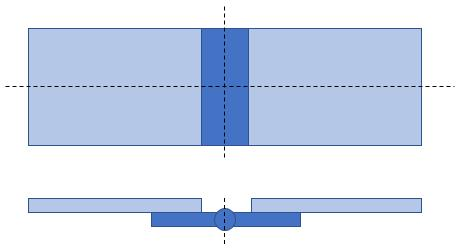
\includegraphics[width=\linewidth]{Bilder/Powerpoint/Schanier}
      \caption{Scharnier}
	  \label{Scharnier}      
      \end{minipage}
\end{figure}

\subsubsection{Futterplatte}

\begin{wrapfigure}{r}{0.5\textwidth}
\vspace{-30pt}
  \begin{center}
    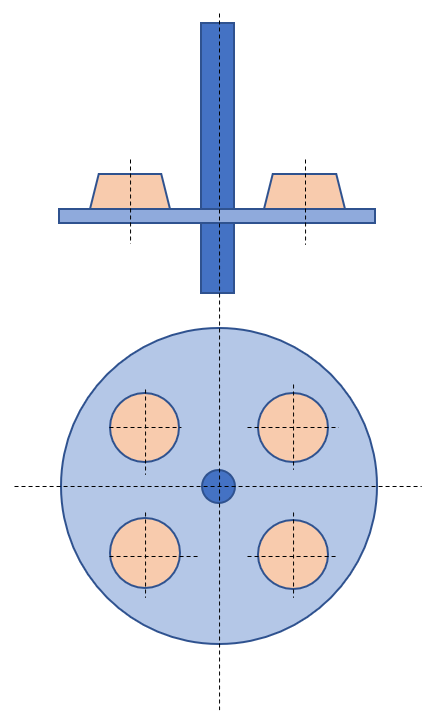
\includegraphics[width=0.20\textwidth]{Bilder/Powerpoint/Futterplatte}
  \end{center}
  \caption{Futterplatte}
  \label{Futterplatte}
  \vspace{-20pt}
\end{wrapfigure}


Nach dem Pressen wird das Futter in die Schüssel gequetscht bzw. es rinnt in die Schüssel. Die Platte hat eine gewisse Anzahl an Schüsseln, je nach Bedarf maximal fünf Schüsseln. Diese sind auf einer Platte platziert, durch den Plattenmittelpunkt geht eine Welle die die Platte nach links und rechts drehen kann. Siehe Abbildung: \ref{Futterplatte} \\


\subsection{Variante 3: Gefrorenes Futter}

In dieser Variante wurde überlegt, ob man das Futter nicht einfrieren kann, dieses danach aus der Gefriertruhe zu holen und zu erwärmen. Der Vorteil hierbei ist, dass keine Schädlinge in das Futter gelangen können da es tiefgefroren ist und es kann die Portionsgröße eingestellt werden wie viel die Katze bekommt da der Benutzer die Menge des Futters selbst bestimmen kann. Weiters müsste man nicht über das Schneide Problem nachdenken, da es eine knifflige Angelegenheit ist die Packung bei jeden Schnitt perfekt zu schneiden. Der große Nachteil ist der Platzbedarf und der hohe Energieverbrauch der Kühltruhe. Auch die Entnahme des Futters aus der Kühltruhe ist kein leichtes Unterfangen. Erstens kann mit Magnetzylindern gearbeitet werden, zur Verschiebung der Abdeckung. Zweitens kann ein Loch aus dem der Greifer das Futter entnimmt und dicht halten muss in die Gefriertruhe geschnitten werden. Falls es undicht ist, wird es darin zu warm, das Futter schmilzt und verdirbt schlussendlich. Hinzuzufügen ist auch noch das Katzen wenn es um Futter geht sehr wählerisch sind und somit wenn das Futter gefroren ist, hat man zu einem  Teil das Kondenswasser des aufgetauten Futters und zum Anderen schmeckt eingefrorenes Essen anders, also nicht so wie es die Katze gewohnt ist.

\section{Aufbauten und Tests}

In diesem Abschnitt der Diplomarbeit wurden Teile der vorne beschriebenen Varianten aufgebaut und verschiedene Tests durchgeführt, um die Funktionalität der Varianten zu gewährleisten. \\

\subsection{Fütterungsexperiment} 

In diesem Experiment wurde getestet wie lange es Dauert bis eine Packung nur mit Hilfe der Schwerkraft ausläuft. Der Beutel wurde nicht extra erwärmt und wird nur an den beiden unteren Ecken gehalten. Siehe Abbildungen: \ref{Halterung}, \ref{Fütterungs Anfang} 

In der Abbildung: \ref{Fütterungs Mitte} zeigt wie viel nach 5 Minuten von der Packung in den Futterbehälter geflossen ist.

In der Abbildung: \ref{Fütterungs_Ende} sieht man das nach 10 Minuten der Inhalte ganz in der Futterschüssel entleert wurde, dennoch Tropft es nach.


\begin{figure}[H]
   \begin{minipage}[hbt]{.4\linewidth} % [b] => Ausrichtung an \caption
      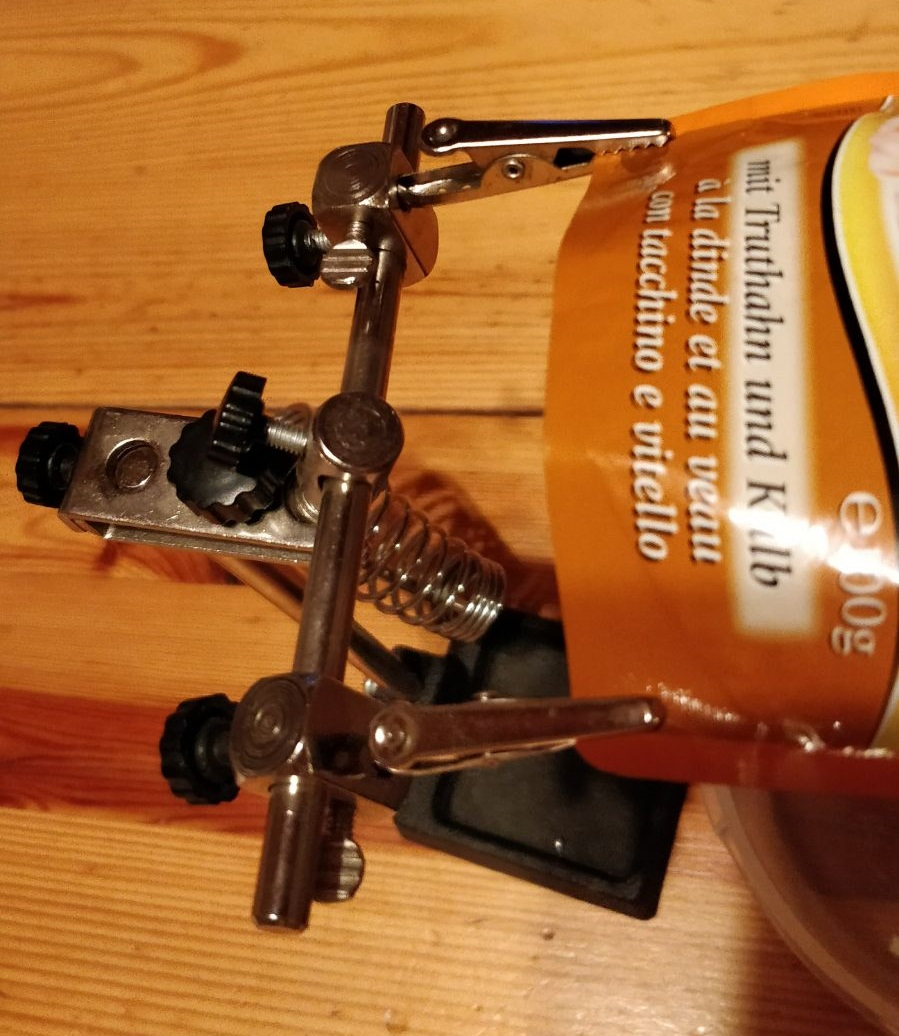
\includegraphics[width=\linewidth]{Bilder/Fuetterungsexperiment/Aufhaengung}
      \caption{Halterung}
      \label{Halterung}
   \end{minipage}
   \hspace{.2\linewidth}% Abstand zwischen Bilder
   \begin{minipage}[hbt]{.4\linewidth} % [b] => Ausrichtung an \caption
      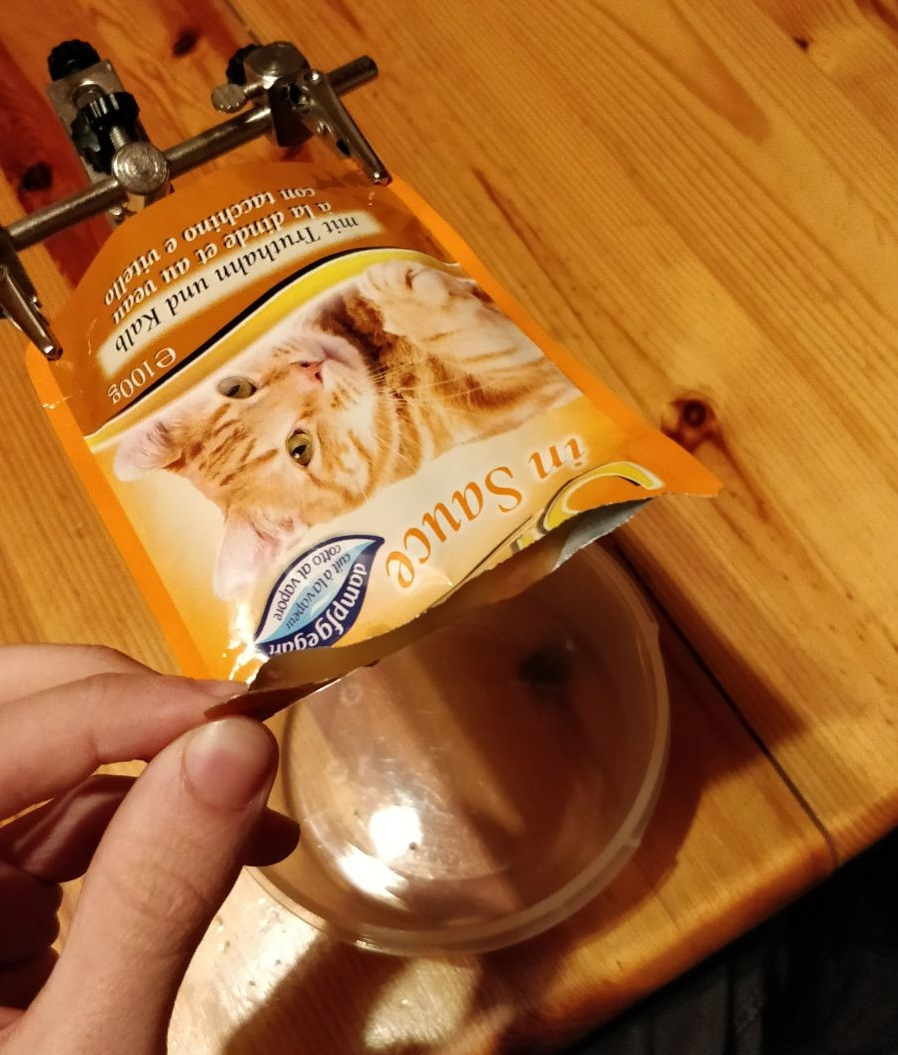
\includegraphics[width=\linewidth]{Bilder/Fuetterungsexperiment/Fuetterungs_Anfang}
      \caption{Entleerung Anfang}
	  \label{Fütterungs Anfang}      
      \end{minipage}
\end{figure}


\begin{figure}[H]
   \begin{minipage}[hbt]{.32\linewidth} % [b] => Ausrichtung an \caption
      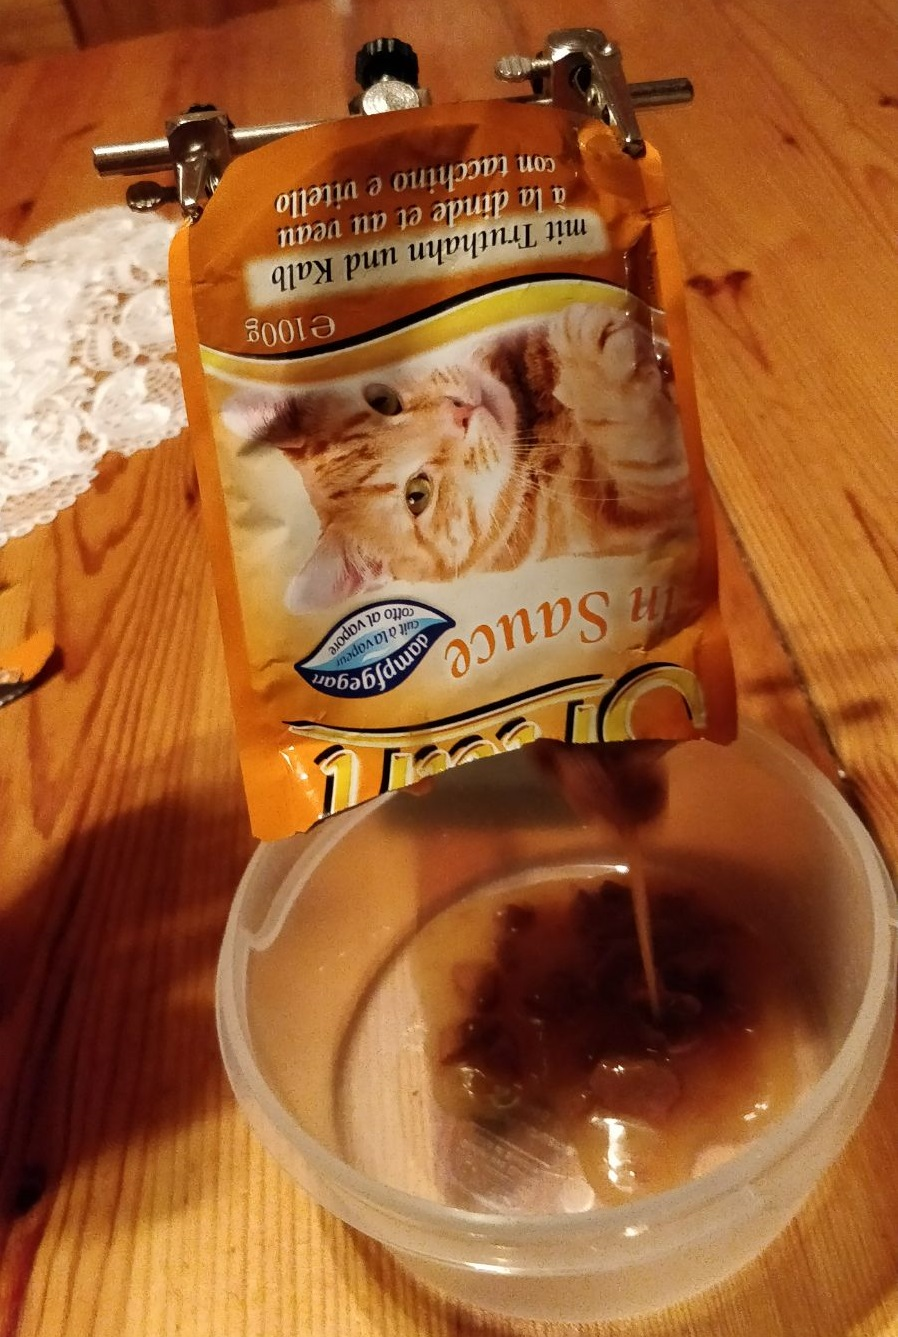
\includegraphics[width=\linewidth]{Bilder/Fuetterungsexperiment/Fuetterungs_Mitte}
      \caption{Entleerung nach 5min}
      \label{Fütterungs Mitte}
   \end{minipage}
   \hspace{.3\linewidth}% Abstand zwischen Bilder
   \begin{minipage}[hbt]{.33 \linewidth} % [b] => Ausrichtung an \caption
     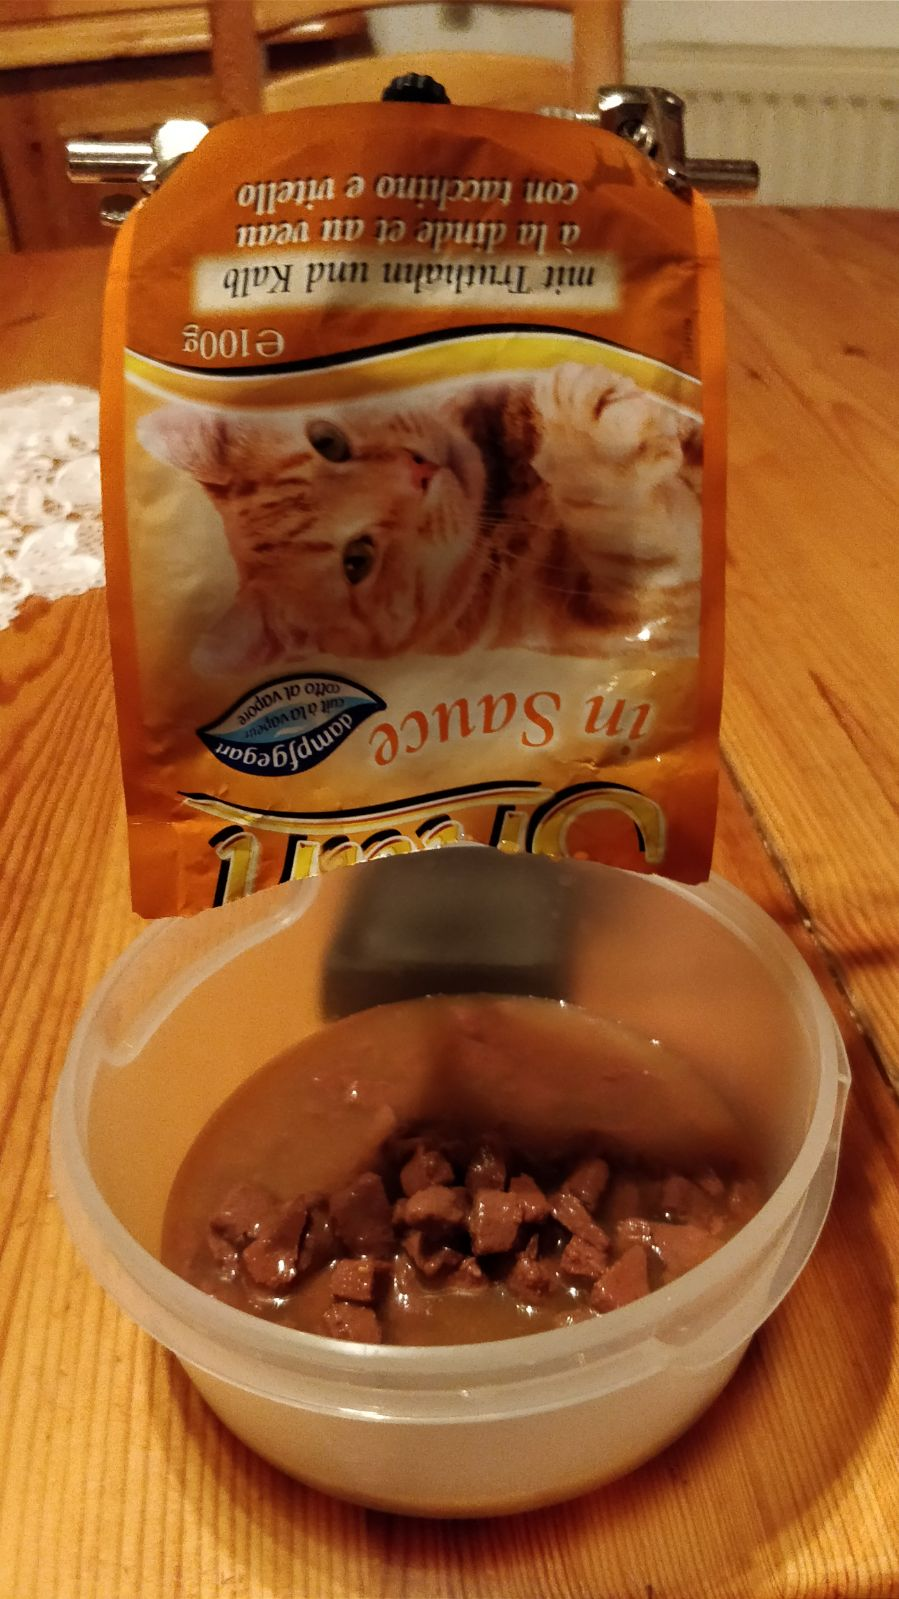
\includegraphics[width=\linewidth]{Bilder/Fuetterungsexperiment/Fuetterungs_Ende}  
      \caption{Entleerung nach 10min}
     \label{Fütterungs_Ende}
   \end{minipage}
\end{figure}

\subsubsection{Schlussfolgerung des Fütterungsexperimentes}

Durch die Beobachtung lässt sich durch das Experiment folgende Schlussfolgerungen treffen: 
\begin{itemize}
\item Durch die leichte Gelee-artige aber eher dünnflüssige Konsistenz des Futters	rinnt es abhängig von der Zeit aus der Packung.
\item Dadurch der ganze Inhalt leicht gleitet kann ohne Probleme durch eine Walze das restlich Futter ausgepresst werden.
\item Durch das Eigengewicht und der Schwerkraft wird der Entleerungsprozess erleichtert.
\end{itemize} 

\subsection{Schneideversuch 1.Art der 1.Variante}

Schnitt anhand einer praxischen Anwendung dargestellt. Der Beutel wird mithilfe einer Papierschneidemaschine geschnitten. Siehe Abbildungen: \ref{Einlegen}, \ref{Anfangsschnitt}, \ref{Endschnitt}

\begin{figure}[H]
   \begin{minipage}[hbt]{.3\linewidth} % [b] => Ausrichtung an \caption
      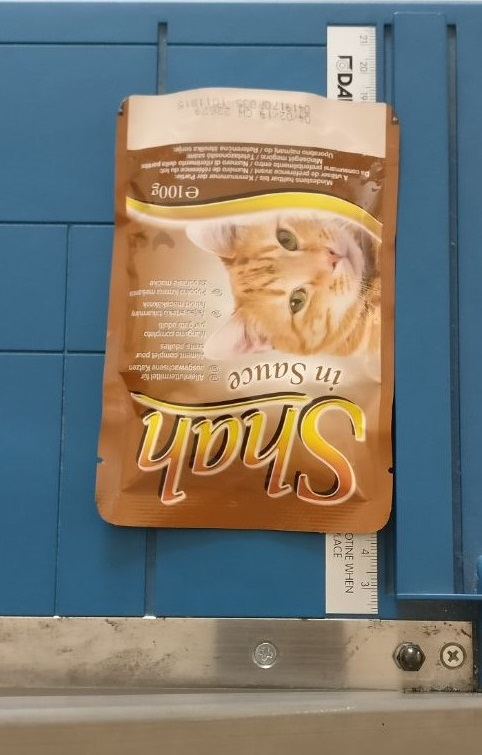
\includegraphics[width=\linewidth]{Bilder/Schneideversuch_1.Art/Einlegen}
      \caption{Einlegen}
      \label{Einlegen} 
   \end{minipage}
   \hspace{.2\linewidth}% Abstand zwischen Bilder
   \begin{minipage}[hbt]{.5\linewidth} % [b] => Ausrichtung an \caption
      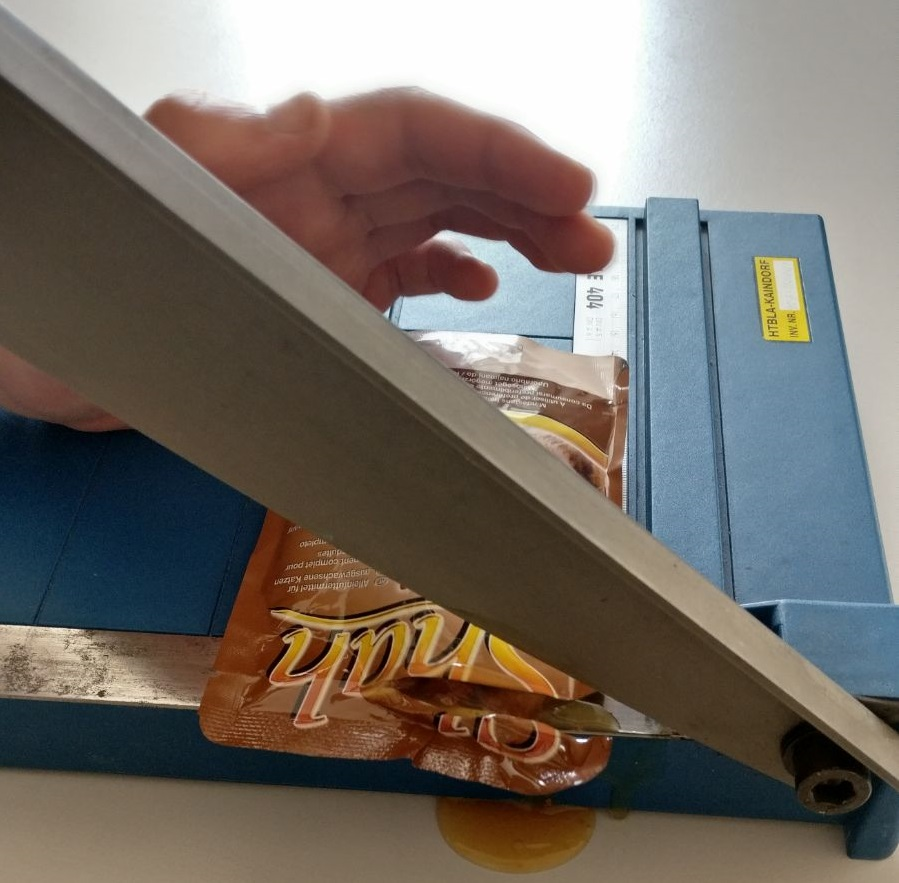
\includegraphics[width=\linewidth]{Bilder/Schneideversuch_1.Art/Anfangsschnitt}
      \caption{Anfangsschnitt}
      \label{Anfangsschnitt} 
   \end{minipage}
\end{figure}

\begin{figure}[H]
\begin{center}
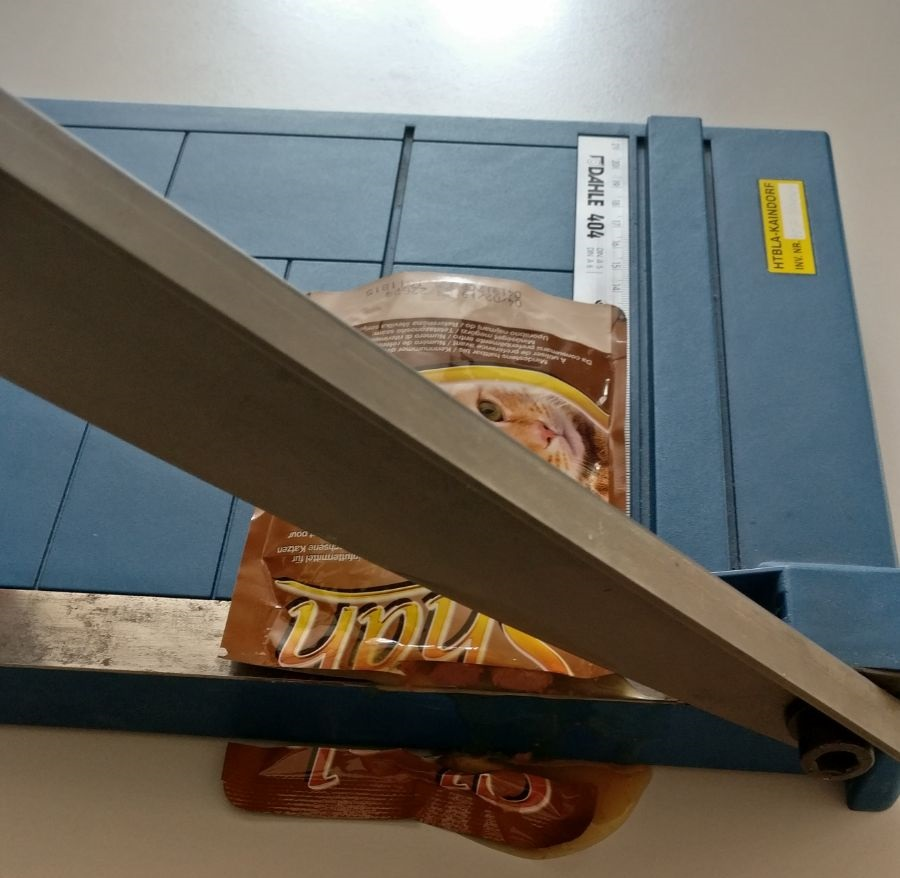
\includegraphics[width=7cm]{Bilder/Schneideversuch_1.Art/Endschnitt}
\caption{Endschnitt}
\label{Endschnitt} 
\end{center}
\end{figure}
\subsubsection{Schlussfolgerung des Schneideversuchs 1.Art der 1.Variante }

Diese ist von den beiden Schneidevarianten die bevorzugte und wurde durch  abwiegen der pro und kontra ausgewählt bzw. Tests ausgewählt.

In den folgenden Punkten sind die Ergebnisse von der ersten Variante aufgelistet:

\begin{itemize}
\item Durch den hohen Anpressdruck der Schneide an die Schneidplatte ließ sich die Packung vollständig öffnen.
\item Es gelang beim 1.Versuch mit nur einen durchgehenden Schnitt.
\item Die lange Klinge machte auch keine Problem indem die Packung zwischen der Schneidfläche und Klinge gelang und diese auseinander drückt.
\item Durch die vom Futterhersteller vorgegebene Einkerbung kann mit realtiv wenig Kraft eine Rissfortpflanzung hervorrufen(genauere Beschreibung unter Variante 1, Führen zur Schneidplatte).
\item Konnte wie beim Greifer ein genaues Einspannen hervorrufen.
\end{itemize} 

\subsection{Schneideversuch 2.Art der 1.Variante}

Mit einem Metallwerkzeug mit Wellenschliffartiger Kante wird der Futterbeutel entlang der Oberseite aufgeschnitten. Um die Packung vollständig geöffnet zu haben, mussten mehrere Schnitte verwendet werden. Siehe Abbildung: \ref{Schneidemittel}\\
In der Abbildung: \ref{Nach 3 Schnitten} erkennt man wie offen die Packung nach 3 Schnitten ist.\\
In der Abbildung: \ref{Nach 6 Schnitten} erkennt man wie offen die Packung nach 6 Schnitten ist.\\
In der Abbildung: \ref{Nach 9 Schnitten} wurde die Packung nach 9 Schnitten vollständig geöffnet.

\begin{figure}[H]
   \begin{minipage}[hbt]{.3\linewidth} % [b] => Ausrichtung an \caption
      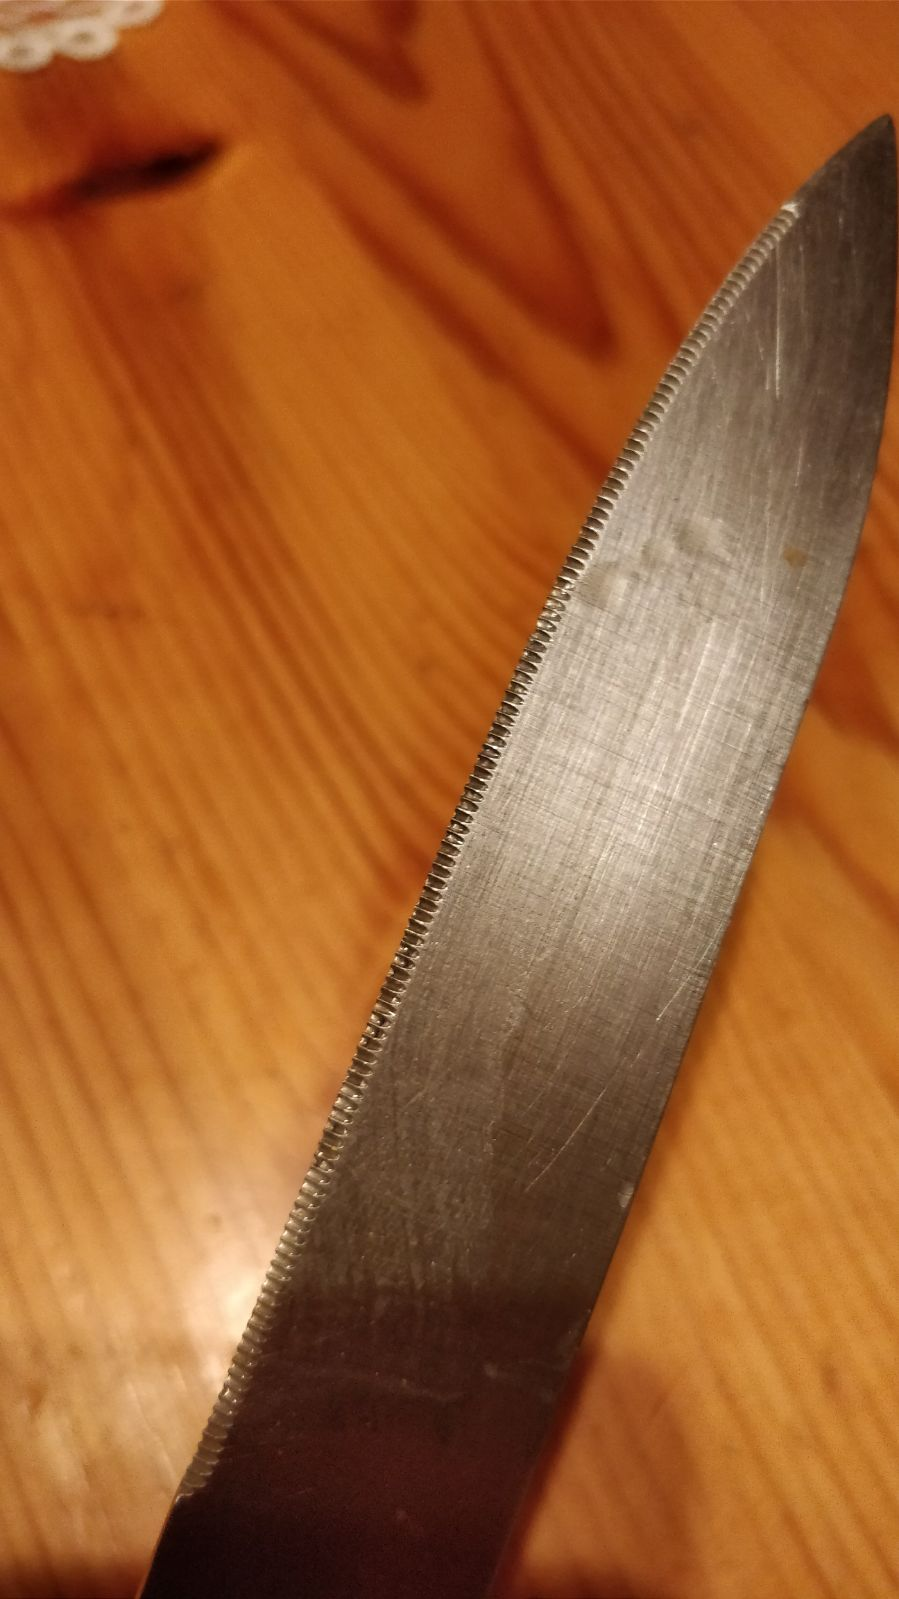
\includegraphics[width=\linewidth]{Bilder/Schneideversuch_2.Art/Schneidemittel}
      \caption{Schneidemittel}
      \label{Schneidemittel} 
   \end{minipage}
   \hspace{.4\linewidth}% Abstand zwischen Bilder
   \begin{minipage}[hbt]{.3\linewidth} % [b] => Ausrichtung an \caption
      
\includegraphics[width=\linewidth]{Bilder/Schneideversuch_2.Art/Anfangsschnitt}
      \caption{Anfangsschnitt 2.Art}
      \label{Nach 3 Schnitten}
   \end{minipage}
\end{figure}


\begin{figure}[H]
   \begin{minipage}[hbt]{.4\linewidth} % [b] => Ausrichtung an \caption
      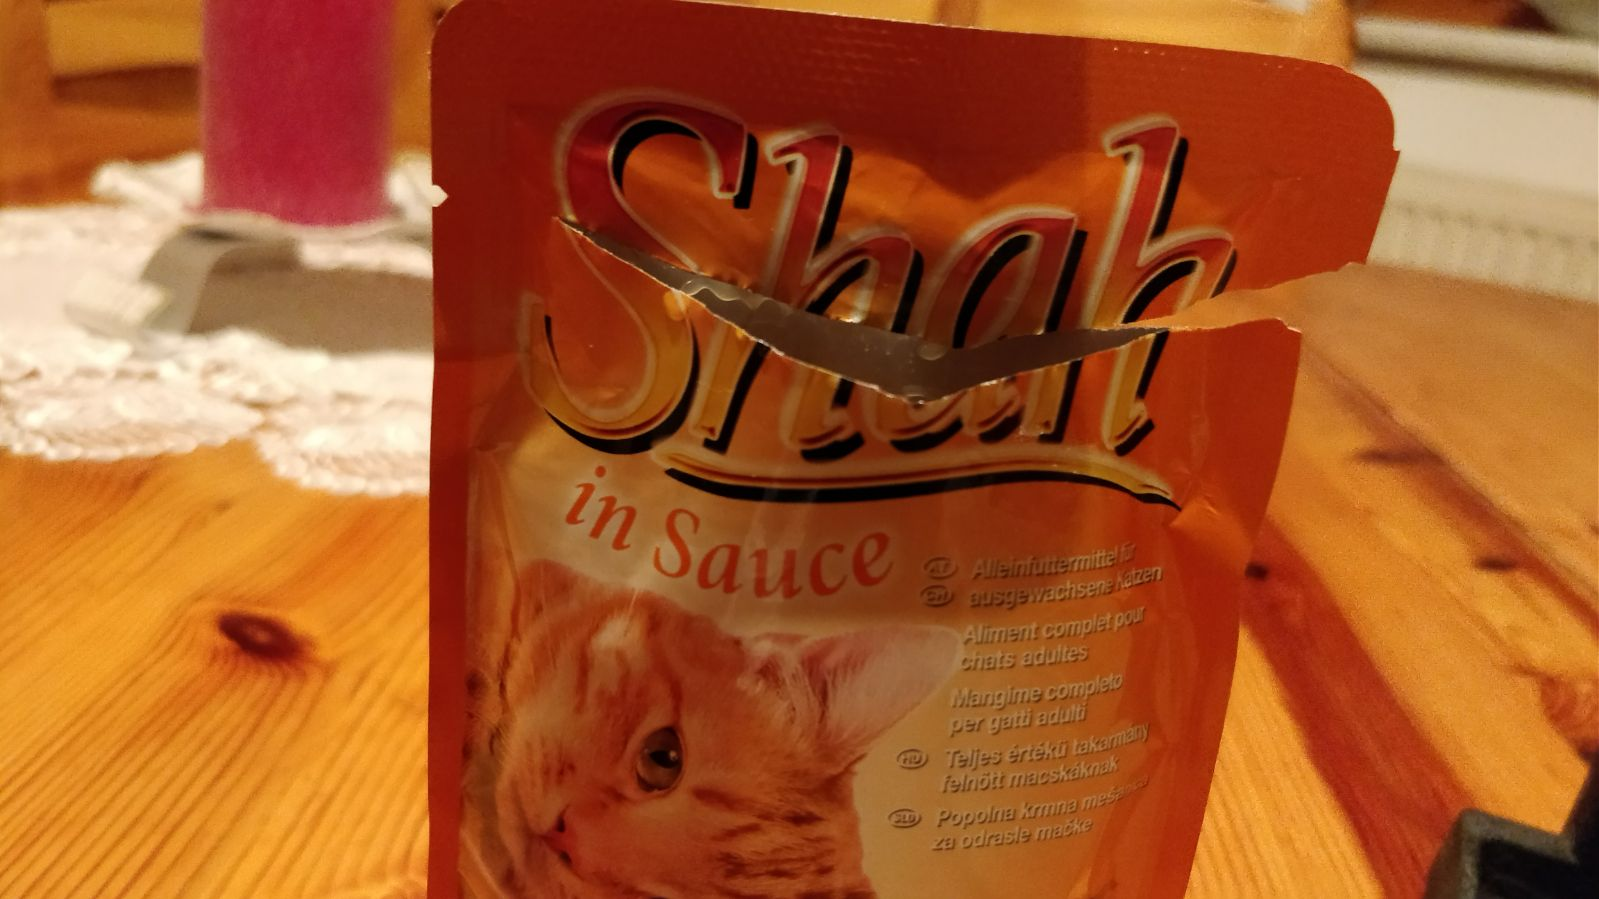
\includegraphics[width=\linewidth]{Bilder/Schneideversuch_2.Art/Mittelschnitt}
      \caption{Mittelschnitt 2.Art}
      \label{Nach 6 Schnitten}
   \end{minipage}
   \hspace{.2\linewidth}% Abstand zwischen Bilder
   \begin{minipage}[hbt]{.4\linewidth} % [b] => Ausrichtung an \caption
      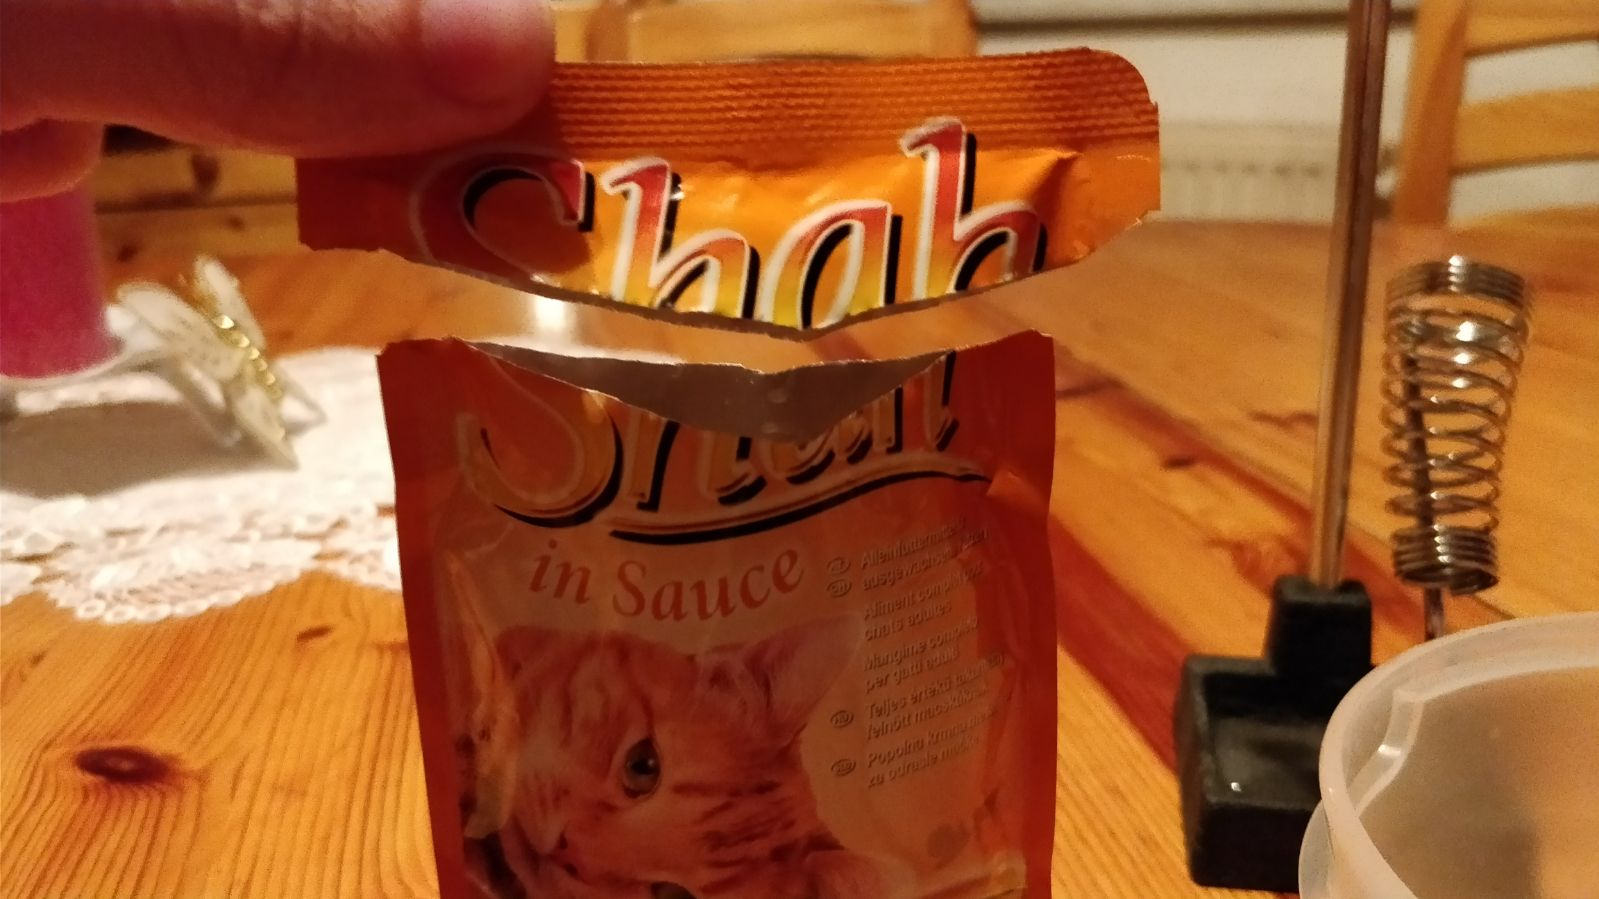
\includegraphics[width=\linewidth]{Bilder/Schneideversuch_2.Art/Endschnitt}
      \caption{Endschnitt 2.Art}
      \label{Nach 9 Schnitten}
   \end{minipage}
\end{figure}

\subsubsection{Schlussfolgerung des Schneideversuchs 2.Art der 1.Variante }

In den folgenden Punkten werden die Ergebnisse und auch Alternativen der zweiten Variante aufgelistet:

\begin{itemize}
\item Falls die Packung nicht genau eingespannt ist kann durch die zackige Schneide kein guter Schnitt vollbracht werden, da die Klinge nicht schneidet sondern reißt.
\item Wenn auf diese Weise der Schneidemechanismus gelöst wäre sollte, müsste man die mit einer anderen Alternative lösen. Das wäre eine Sägezahnrad das mit eine Elektromotor angetrieben wird.
\item Kein gerader Schnitt erwartet, wegen das reißen der Verpackung, hervorgerufen durch die zackige Klinge(würden funktionieren mit zusätzlicher Sicherung). 
\end{itemize} 
\newpage
\subsection{Dichtheitsexperiment der Hebelklemme}


\begin{wrapfigure}{r}{0.5\textwidth}
\vspace{-20pt}
  \begin{center}
    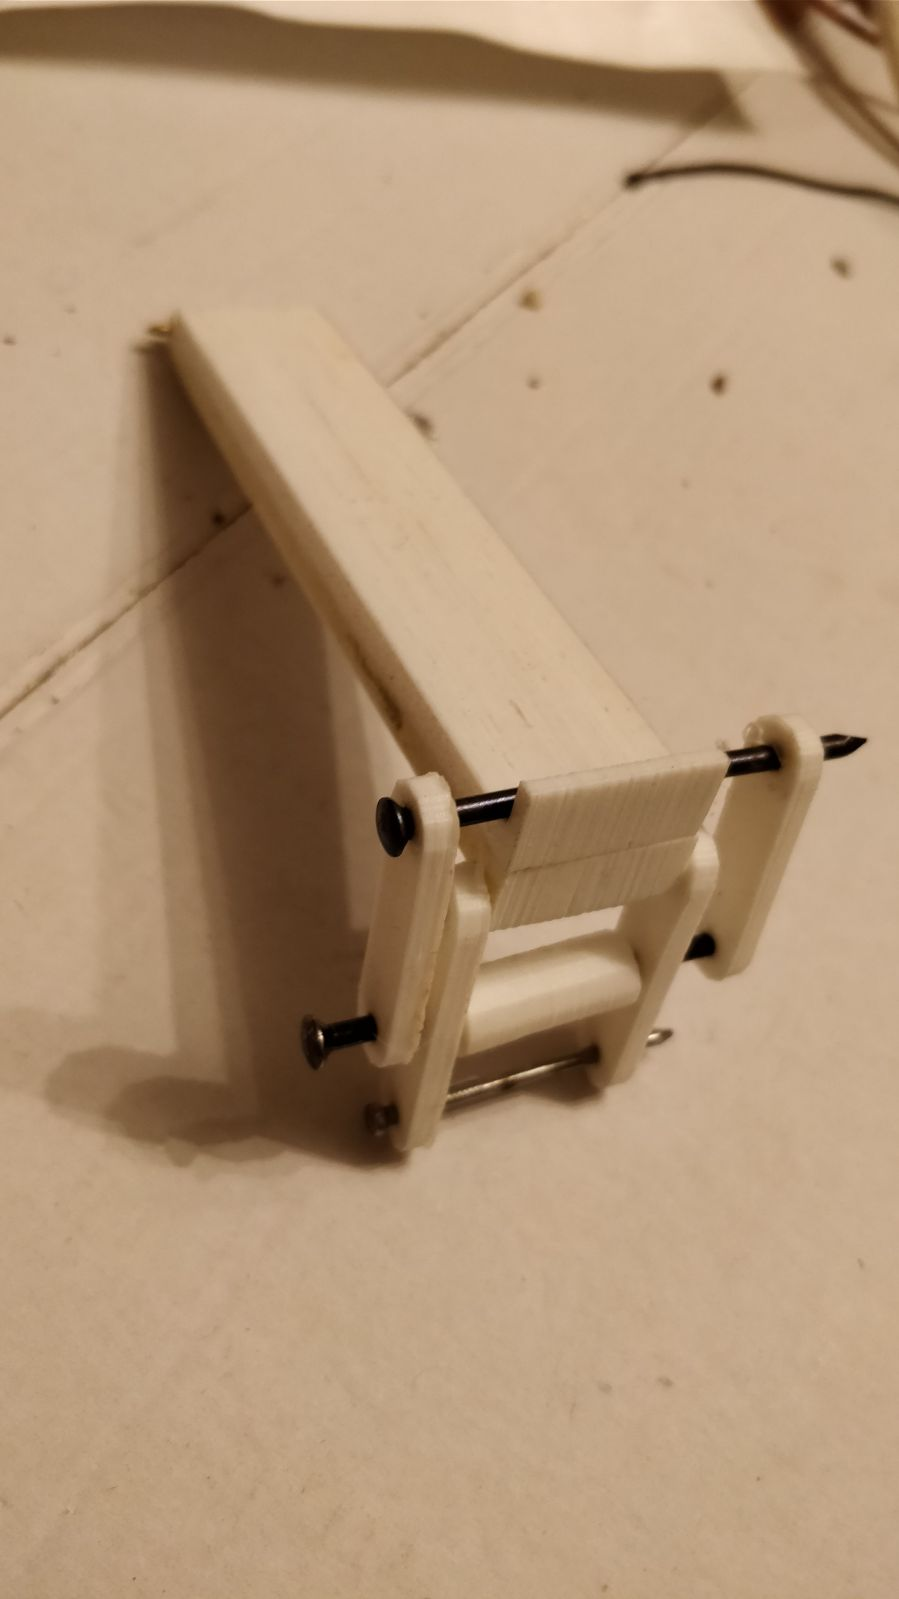
\includegraphics[width=0.22\textwidth]{Bilder/Dichtheitsexperiment/Klemme}
  \end{center}
  \caption{3D-Klemme}
  \label{3D-Klemme}
  \vspace{-20pt}
\end{wrapfigure}

Die für unsere Maschine entscheidende Klemme wurde 3D gedruckt und getestet wie sich die Packung nach fünf Tagen verhält. Von der Klemme wurde nur die Umrandung der einzelnen Teile gedruckt das heißt die Teile sind in der Mitte hohl und dehnbarer als massive Teile für die Klemme. Im Bild: \ref{3D-Klemme} erkennt man den ersten Prototypen der Klemme. Die gedruckten Teile werden mit 1,5mm dicke Nägel verbunden. Die Klemme wird im richtigen Modell mit Metall gebaut und die Nägel werden durch passende Stifte ersetzt.\\

Die Aufgabe der Klemme war, diese fünf Tage senkrecht aufzuhängen und die Klemme auf stärken und schwächen zu Prüfen.\\

Tag 1: Die Klemme wurde samt der Packung senkrecht Aufgehängt und an den von Futterhersteller vorgegeben Schneidepunkt aufgeschnitten. Siehe Abbildung: \ref Der erste Eindruck war die Klemme hält dicht ohne menschliche Einflüsse. Sobald die Klemme wenig gepresst wurde ran die Flüssigkeit aus der Klemme, weil diese nicht massiv bzw. stabil genug ist. Die beiden längeren Flächen die über die Packung gelegt werden bogen sich durch die menschliche Einwirkung und den inneren der Packung auseinander. Dennoch war die Klemme, wenn sie sich in Ruhelage befindet dicht. Siehe Abbildung: \ref{Klemme_Tag_1}.

\begin{figure}[H]
   \begin{minipage}[hbt]{.5\linewidth} % [b] => Ausrichtung an \caption
      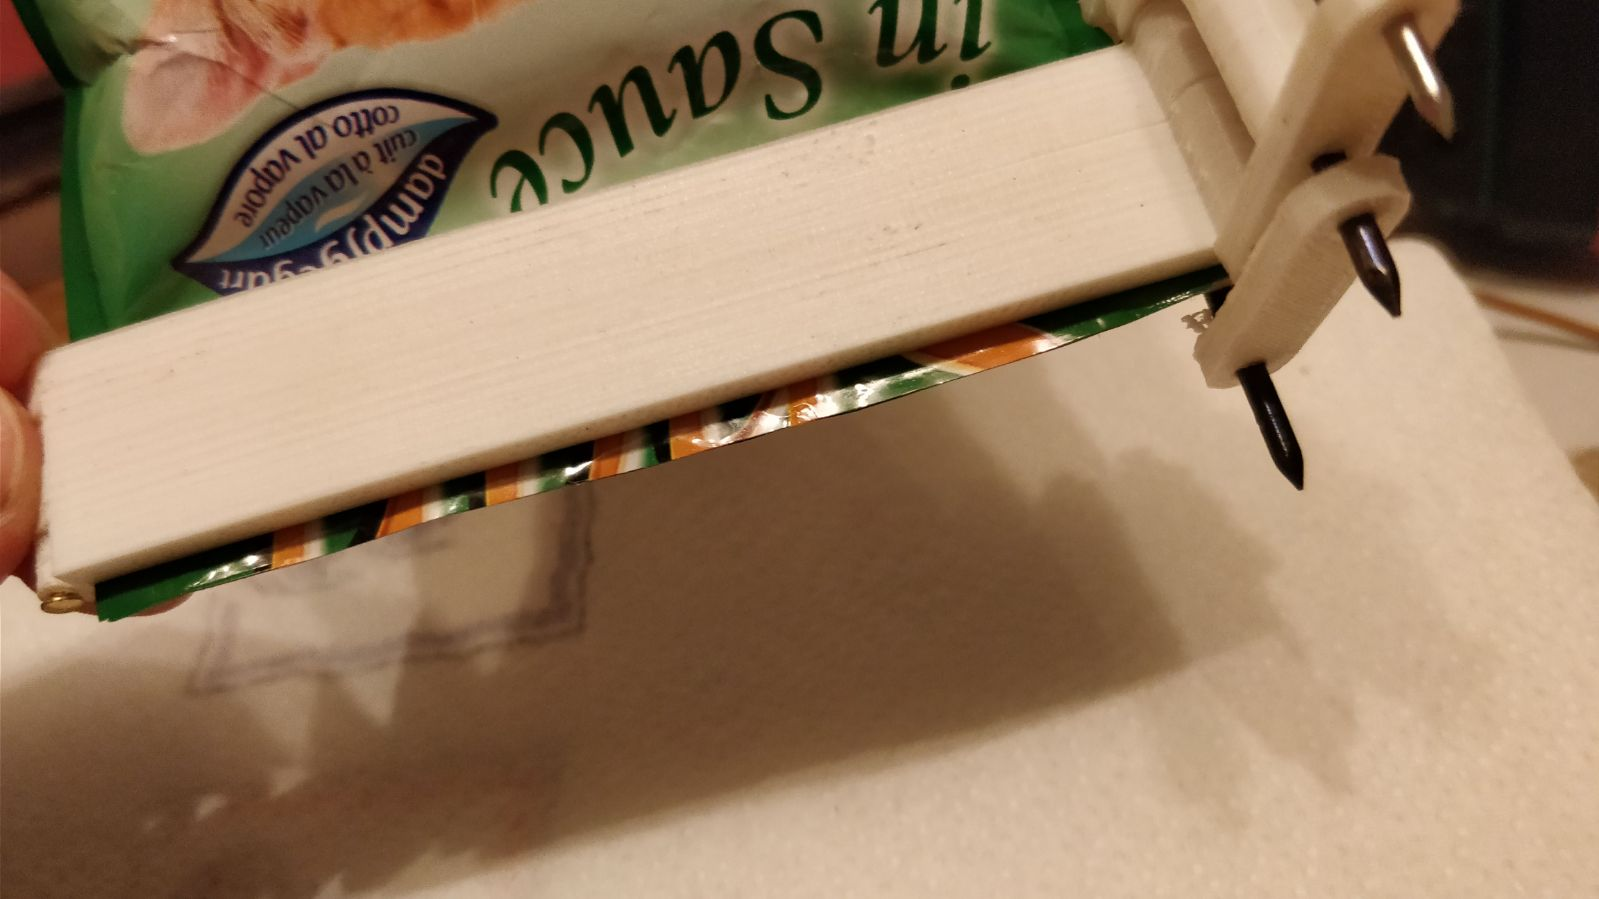
\includegraphics[width=\linewidth]{Bilder/Dichtheitsexperiment/Probe}
      \caption{Klemmen Probe}
      \label{Klemmen_Probe} 
   \end{minipage}
   \hspace{.2\linewidth}% Abstand zwischen Bilder
   \begin{minipage}[hbt]{.3\linewidth} % [b] => Ausrichtung an \caption
      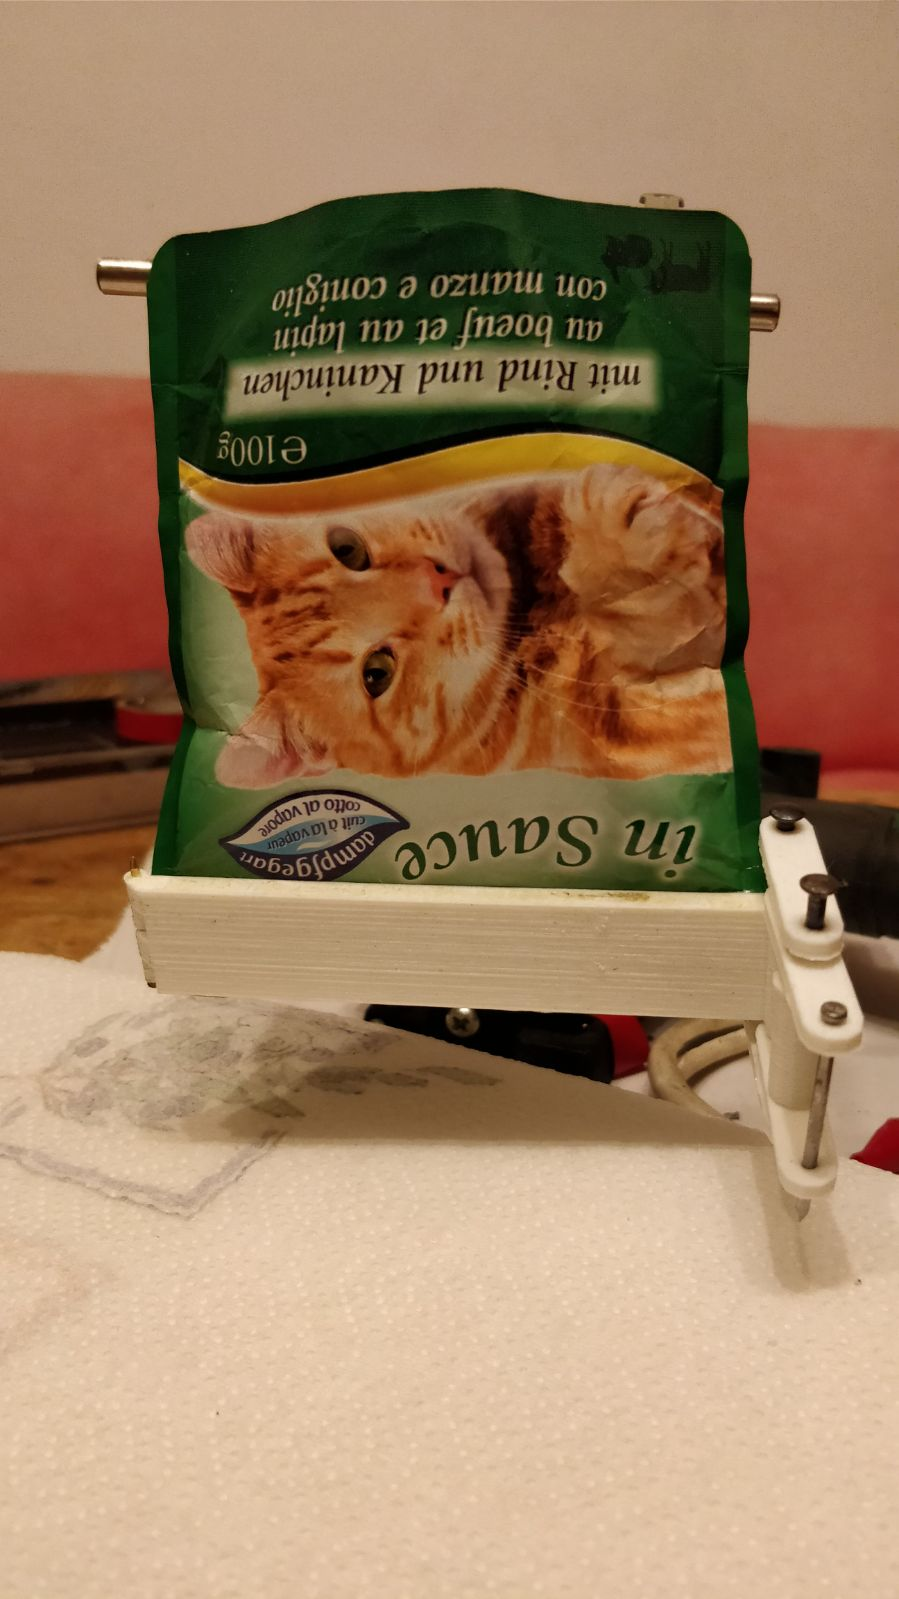
\includegraphics[width=\linewidth]{Bilder/Dichtheitsexperiment/Tag_1}
      \caption{Klemme Tag 1}
      \label{Klemme_Tag_1}
   \end{minipage}
\end{figure}

Tag 2: Zur Überprüfung ob die Packung dicht hält wurde eine weiße Unterlage darunter geschoben in diesem Fall ein Blatt-Küchenrolle. Auch hier sieht man durch einen bildlichen Beweis das unter der Packung nichts verschmutzt ist. Siehe Abbildung: \ref{Klemme_Tag_2}. \\

Tag 3: Das gleiche Resultat wie am Tag 1 und 2. Siehe Abbildung: \ref{Klemme_Tag_3}.

\begin{figure}[H]
   \begin{minipage}[hbt]{.3\linewidth} % [b] => Ausrichtung an \caption
      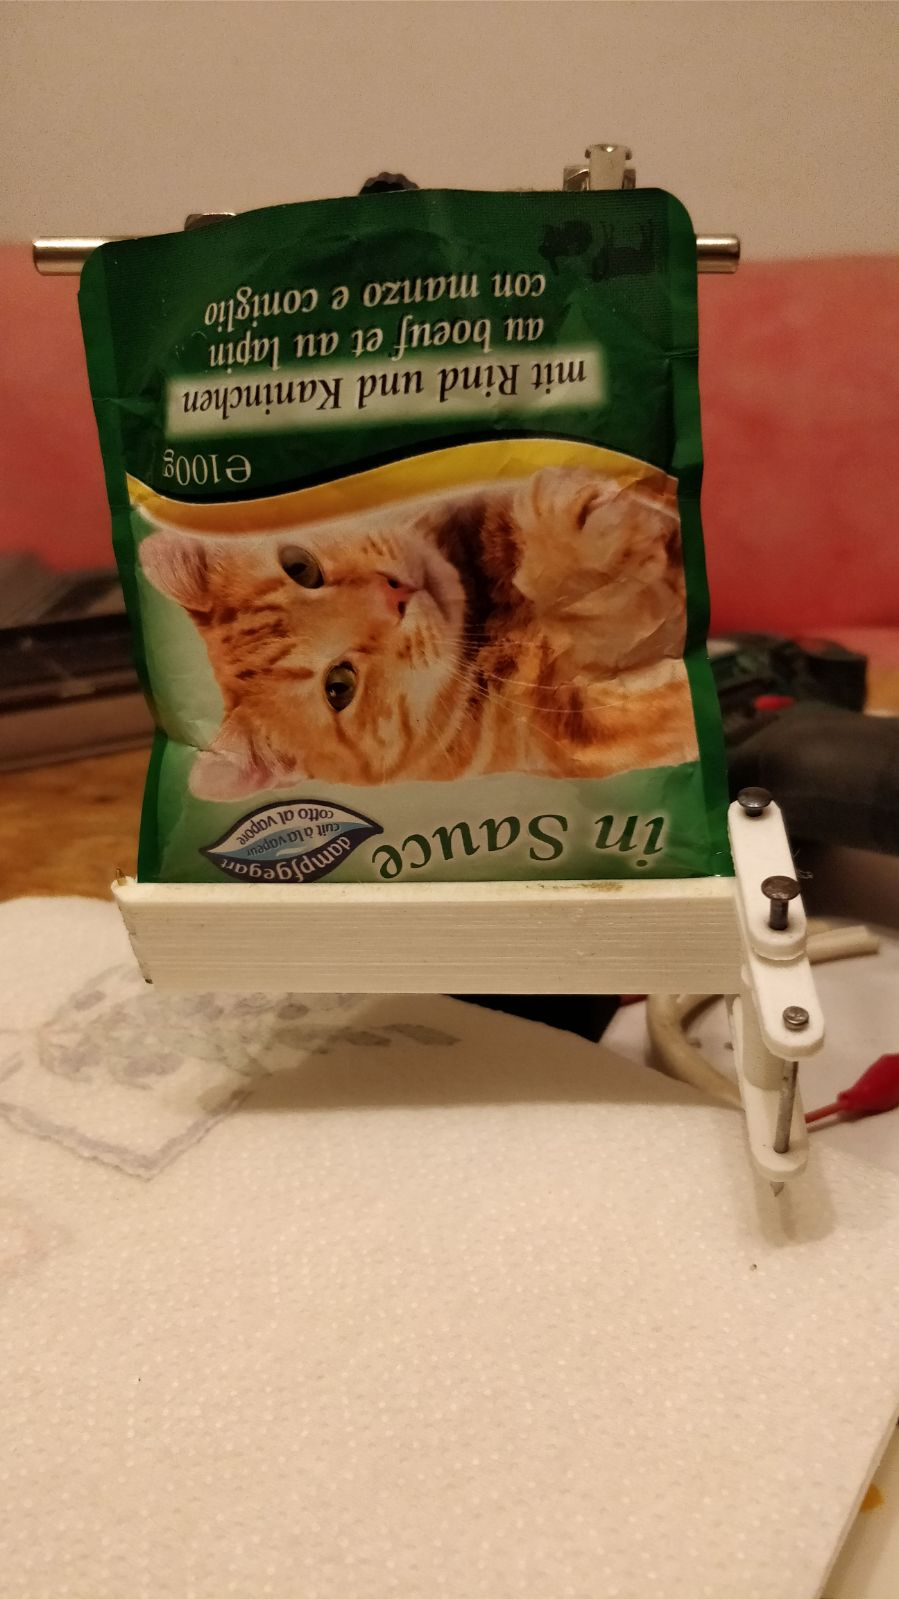
\includegraphics[width=\linewidth]{Bilder/Dichtheitsexperiment/Tag_2}
      \caption{Klemme Tag 2}
      \label{Klemme_Tag_2} 
   \end{minipage}
   \hspace{.3\linewidth}% Abstand zwischen Bilder
   \begin{minipage}[hbt]{.3\linewidth} % [b] => Ausrichtung an \caption
      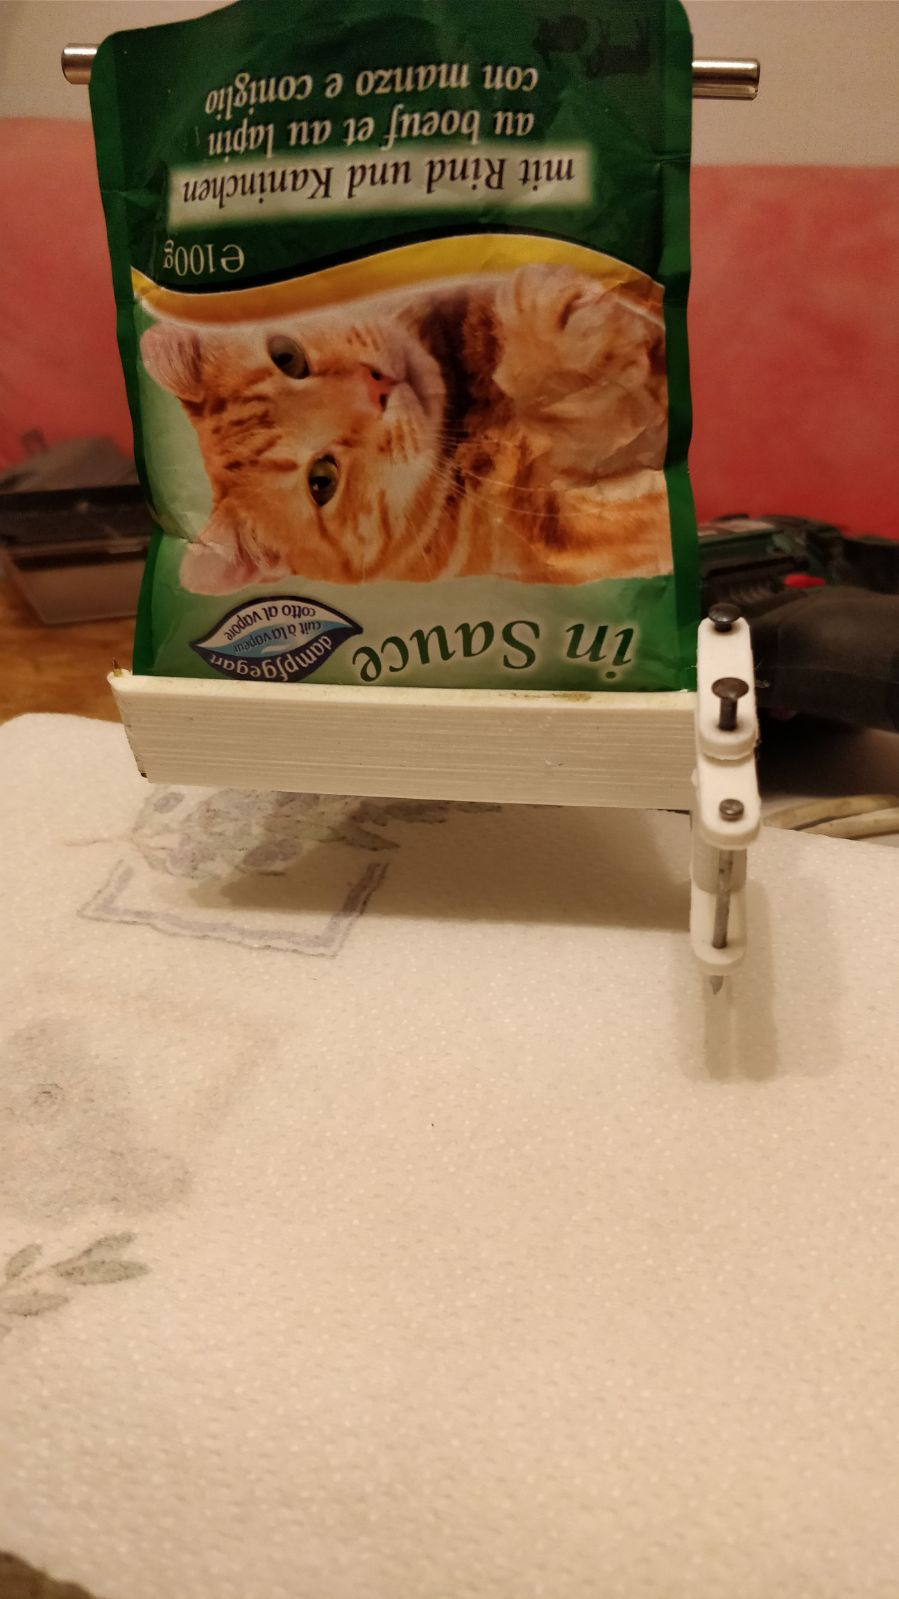
\includegraphics[width=\linewidth]{Bilder/Dichtheitsexperiment/Tag_3}
      \caption{Klemme Tag 3}
      \label{Klemme_Tag_3}
   \end{minipage}
\end{figure}

Tag 4: Wie am Bild \ref{Klemme_Tag_4} zu sehen war am vierten Tag auch keine Flüssigkeit am Tuch. Siehe Abbildung: \ref{Klemme_Tag_4}.\\ 

Tag 5: Der Beweiß ist vollbracht. Die ganzen fünf Tage die der Benutzer im Urlaub ist hält auch die in stabilere Klemme dicht. Siehe Abbildung: \ref{Klemme_Tag_5}.

\begin{figure}[H]
   \begin{minipage}[hbt]{.3\linewidth} % [b] => Ausrichtung an \caption
      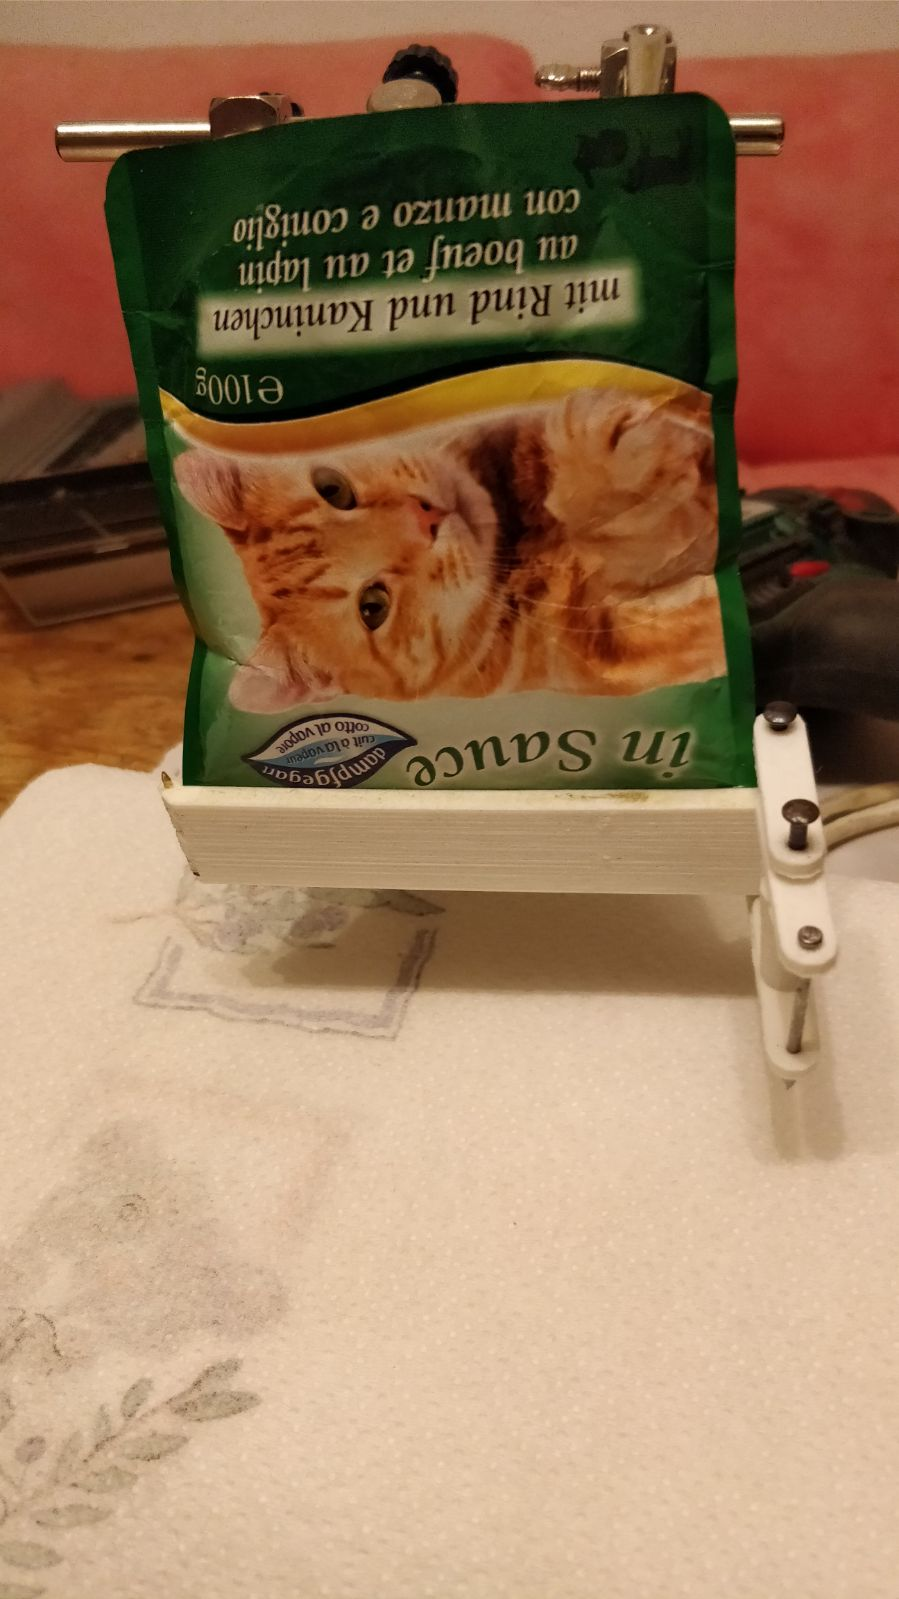
\includegraphics[width=\linewidth]{Bilder/Dichtheitsexperiment/Tag_4}
      \caption{Klemme Tag 4}
      \label{Klemme_Tag_4} 
   \end{minipage}
   \hspace{.3\linewidth}% Abstand zwischen Bilder
   \begin{minipage}[hbt]{.3\linewidth} % [b] => Ausrichtung an \caption
      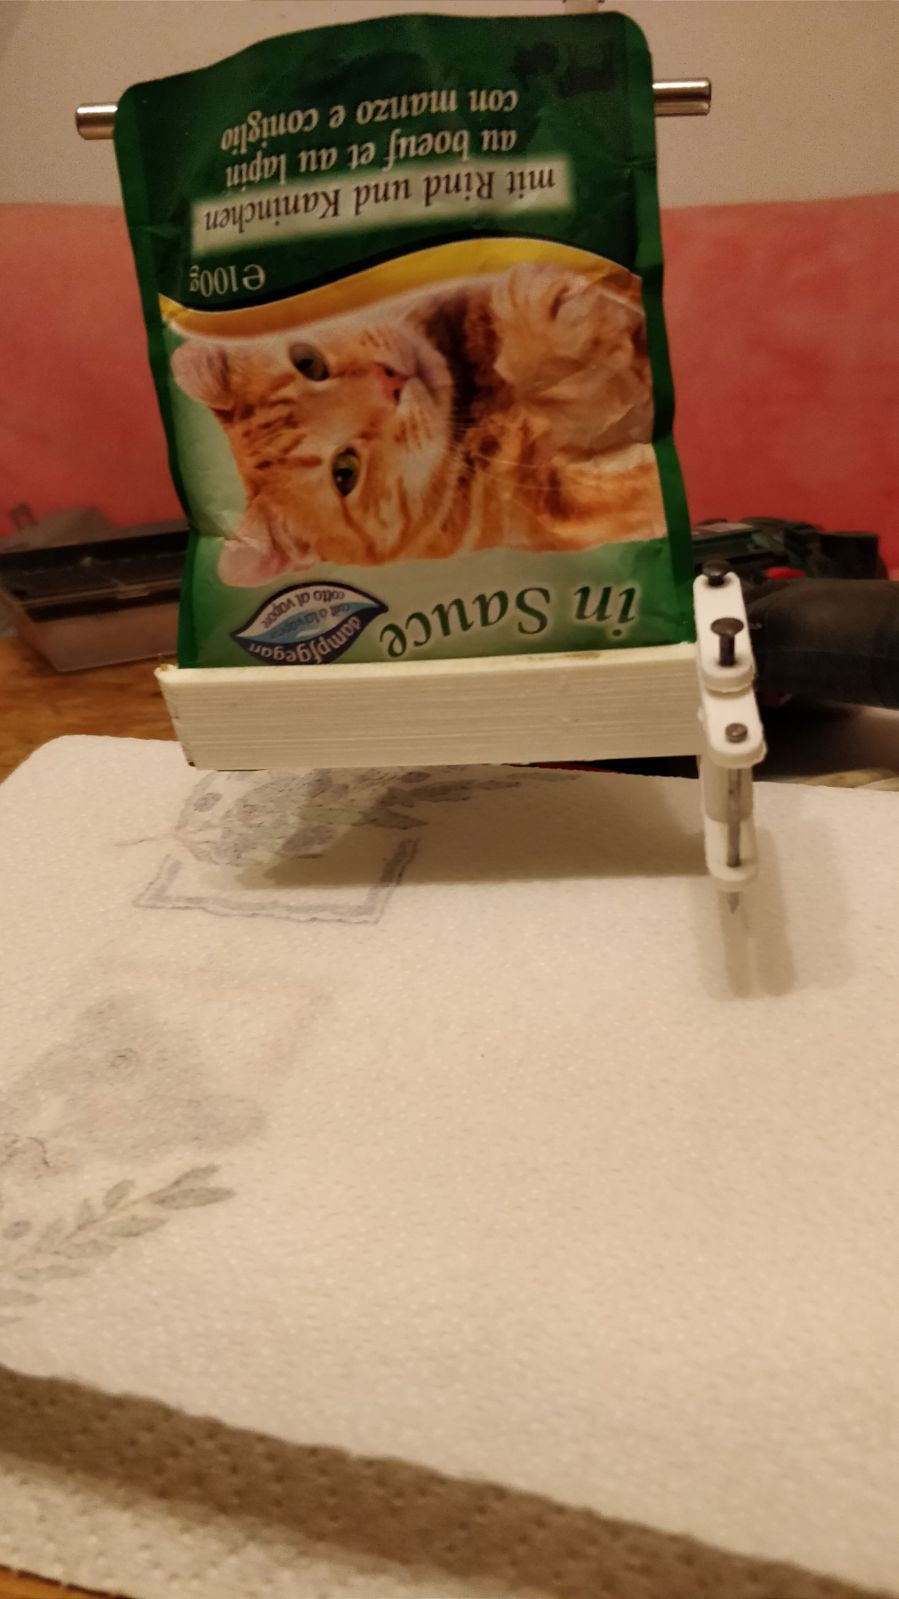
\includegraphics[width=\linewidth]{Bilder/Dichtheitsexperiment/Tag_5}
      \caption{Klemme Tag 5}
      \label{Klemme_Tag_5}
   \end{minipage}
\end{figure}

\section{Vergleich der Varianten}

In diesem Kapitel der Diplomarbeit werden sämtliche Ideen Schemenhaft gezeichnet und erklärt.
 
\subsection{Klemmen}

Es wurden verschieden Varianten durchdacht auf welche Wege die Packung Luftdicht verschlossen werden kann. Dabei sind die folgenden Mechanismen entstanden.

\subsubsection{Einfache Klemme}

\begin{wrapfigure}{r}{0.5\textwidth}
\vspace{-20pt}
  \begin{center}
    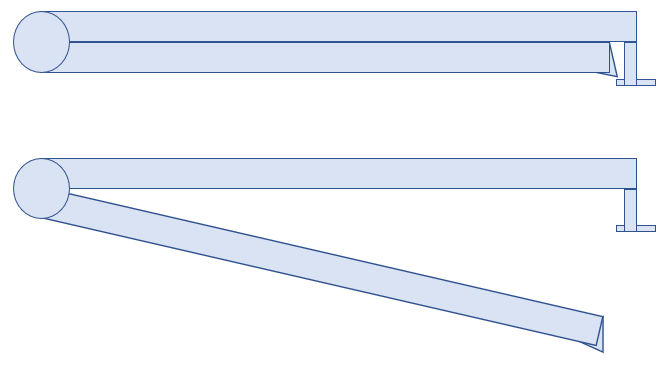
\includegraphics[width=0.32\textwidth]{Bilder/Powerpoint/Einfach_Klemme}
  \end{center}
  \caption{Einfache Klemme}
  \label{Einfache Klemme}
  \vspace{-10pt}
\end{wrapfigure}

Die einfach Klemme ist für gewöhnliche Verpackungen gut zu nutzen jedoch ist sie für unsere Variante nicht zu gebrauchen, weil Kunstoff nicht so stabil wie Metall ist.Drückt die Kunststoffklemme die Packung an manchen Stellen zu wenig zusammen und an diesen Stellen kann Flüssigkeit austreten. Außerdem hält sie bei Zugbelastung nur wenig stand. Siehe Abbildung: \ref{Einfache Klemme}

\subsubsection{Hebel Klemme} 

\begin{wrapfigure}{r}{0.5\textwidth}
\vspace{-30pt}
  \begin{center}
    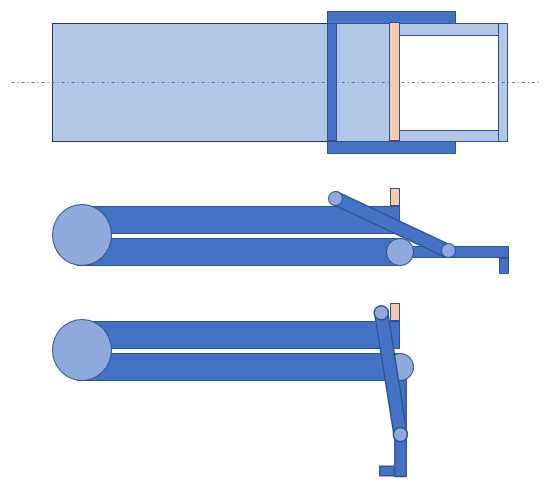
\includegraphics[width=0.32\textwidth]{Bilder/Powerpoint/Hebel_Klemme}
  \end{center}
  \caption{Hebel Klemme}
  \label{Hebel Klemme}
  \vspace{-10pt}
\end{wrapfigure}

Die Hebel Klemme ist für diese Diplomarbeit die bevorzugte Methode, sie kann viel Druck auf die Packung ausüben, sodass keine Flüssigkeit entrinnen kann. Außerdem lässt sich durch den Hebel mit wenig Kraft die Klemme öffnen. Weiters können die Klemmen auf einer Stange aufgesammelt werden und liegen nicht an unerwünschten Positionen an denen man nicht herankommt. Siehe Abbildung: \ref{Hebel Klemme}
 \vspace{40pt}


\subsubsection{Gummiband Klemme}
 
\begin{wrapfigure}{r}{0.5\textwidth}
\vspace{-40pt}
  \begin{center}
    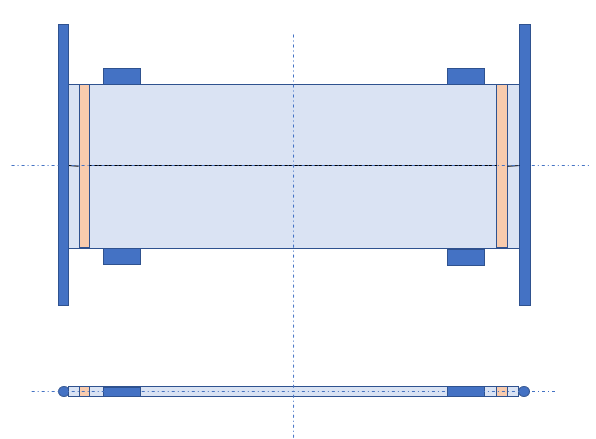
\includegraphics[width=0.30\textwidth]{Bilder/Powerpoint/Gummiband_Klemme}
  \end{center}
  \caption{Gummiband Klemme}
  \label{Gummiband Klemme}
  \vspace{-10pt}
\end{wrapfigure}

Die Gummiband Klemme hat eine starke Klemmkraft, dies Schützt vor dem Aufplatzen der Verpackung. Das Problem dieser Variante ist das das Gummiband spröder werden kann und irgendwann reißen kann, also ein hoher Wartungsaufwand. Die Klemmen kann man auch nicht kontrolliert sammeln und somit sind sie schwerer zugänglich.

\subsection{Klemmen Wahlvariante}

Jede Klemme hat gewisse Vor- und Nachteile. Deshalb wurden alle Varianten miteinander Verglichen und die am besten geeignete Klemme ausgewählt.

Die folgenden Punkte zeigen warum die Hebelklemme für unsere Maschine geeignet ist.

\begin{itemize}
\item Durch den Hebel lässt sich die Klemme leicht öffnen indem das Förderband sich bewegt, die Lasche durch eine Stange eingefädelt wird und diese durch die Bewegung Richtung Walze geöffnet werden soll.
\item Weil die beiden Metallplatten aufeinander pressen hält die Verpackung durch den besonderen Verschluss Luftdicht zusammen (siehe Abbildung: \ref{Hebel Klemme}). 

\end{itemize} 

\subsection{Futterschüsseln}

Bei den Futterschüssel mussten bestimmte Faktoren erfüllt werden bzw. auf wählerische Katzen abgestimmt werden. Deshalb konnte nicht die einfachst Variante genommen werden die am wenigsten Aufwand benötigt hätte. 

\subsubsection{Drehfutterplatte}

\begin{wrapfigure}{r}{0.5\textwidth}
\vspace{-40pt}
  \begin{center}
    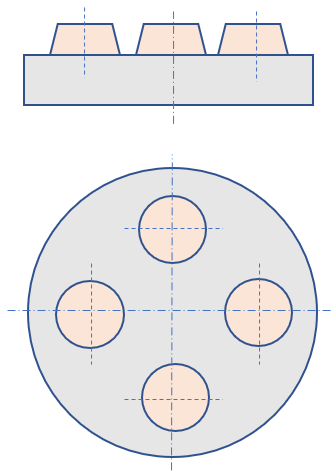
\includegraphics[width=0.25\textwidth]{Bilder/Powerpoint/Drehplatte}
  \end{center}
  \caption{Drehplatte}
  \label{Drehplatte}
  \vspace{-20pt}
\end{wrapfigure}

Die Drehplatte besteht aus fünf Schüsseln man kann pro Schüssel die Katze 2-mal pro Tag füttern z.B morgens und abends. Dadurch hat die Katze jeden Tag eine neue Schüssel und falls sie nicht frisst muss sie nicht Hunger leiden. Auf einer Welle wird eine Platte befestigt. 
Darin werden fünf Löcher geschnitten und die Schüssel hinein gelegt. Die Drehplatte wird mit einem Schneckengewinde in die gewünschten Position gebracht. Siehe Abbildung: \ref{Drehplatte} 

\subsubsection{Futterplatte Zylinder}

\begin{wrapfigure}{r}{0.5\textwidth}
\vspace{-20pt}
  \begin{center}
    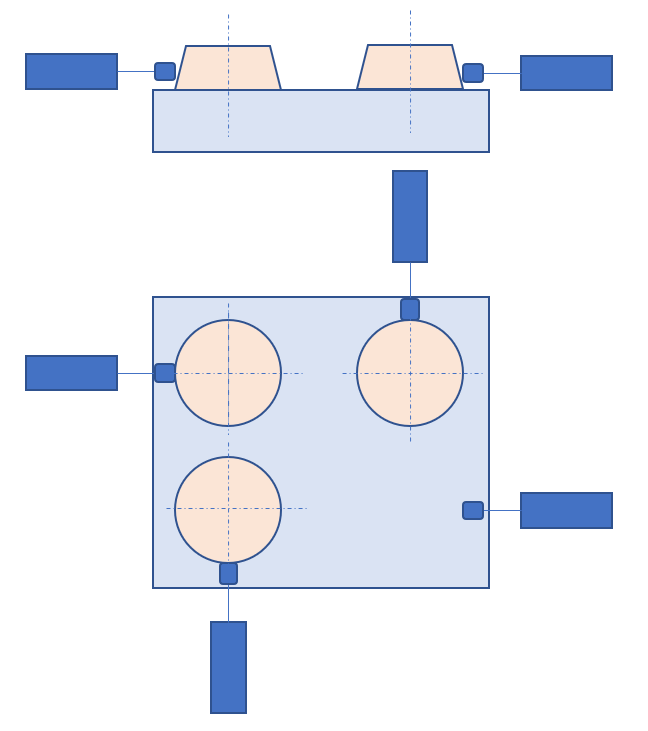
\includegraphics[width=0.32\textwidth]{Bilder/Powerpoint/Platte_Zylinder}
  \end{center}
  \caption{Platte Zylinder}
  \label{Platte Zylinder}
\vspace{-60pt}
\end{wrapfigure}

Die Futterplatte mit Zylinder ist die umständlichste Variante. Es ist eine viereckige Platte auf der Schienen für das schieben der Futterschüsseln platziert sind. Diese werden von Magnetzylindern angeschoben. Der Nachteil hierbei ist, dass viele Bauteile benötigt und alle Zylinder müssen zugleich arbeiten um die Futterschüssel zur richtigen Position zu führen. Siehe Abbildung: \ref{Platte Zylinder} 

\newpage


\subsubsection{Platte mit einer Schüssel}

\begin{wrapfigure}{r}{0.5\textwidth}
\vspace{-20pt}
  \begin{center}
    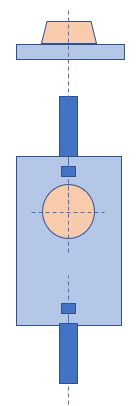
\includegraphics[width=0.10\textwidth]{Bilder/Powerpoint/Einschuessel_platte}
  \end{center}
  \caption{Einschüsselplatte}
  \label{Schüssel Eins}
  \vspace{-10pt}
\end{wrapfigure}

Die Platte mit nur einer Schüssel ist leicht zu realisieren da sie nur wenige Bauteile benötigt. Das wäre zum Einem die Platte auf der die Futterschüssel mit einer Schiene darauf platziert ist und zum Anderen als auch die zwei Magnetzylinder die die Futterschüssel in die Anfangs und Endposition bringt. Jedoch ein großer Nachteil weswegen diese Methode nicht in Frage kommt ist folgendes: Wenn die Katze nach dem Füttern nicht frisst dann bleibt der Inhalt in der Schale und trocknet ein oder es kommt Ungeziefer hinein. Das hat zu Folge das die Schüssel jeden Tag befüllt wird und eventuell übergeht. Siehe Abbildung: \ref{Schüssel Eins} 

\subsection{Futterschüssel Wahlvariante}

Die verschiedenen Futterschüssel haben große Vor- bzw. Nachteil im Platzbedarf und Futterschlüsselanzahl. Diese wurden gründlich durchdacht und zum Folgenden Endschluss gekommen: Die Wahlvariante ist die Drehplatte die Gründe dafür werden in den Punkten erörtert: 

\begin{itemize}
\item Ein großes Thema war die Anzahl der Futterschüsseln, hierbei war es wichtig, dass die Katze jeden Tag eine reine Schüssel zur Verfügung hat.
\item Die Schüsseln sollten leicht zu entfernen sein und die Oberfläche der Platte ebenfalls leicht zu reinigen sein.
\item Dadurch die Platte auf einer Welle sitzt lässt die sich durch den Motor in die Befüll- bzw. Fütterungsposition bringen.
\end{itemize} 

\subsection{Futtermagazine}

Diese Futtermagazine waren für die 1.Variante relevant, bei diesen war es wichtig die Packungen so einfach wie möglich in die Schneideposition zu bringen. Dies sollte ohne Schwierigkeiten bzw. einem zu langen Weg erfolgen. 

\subsubsection{Futtermagazin Horizontal}

\begin{wrapfigure}{r}{0.5\textwidth}
\vspace{-40pt}
  \begin{center}
    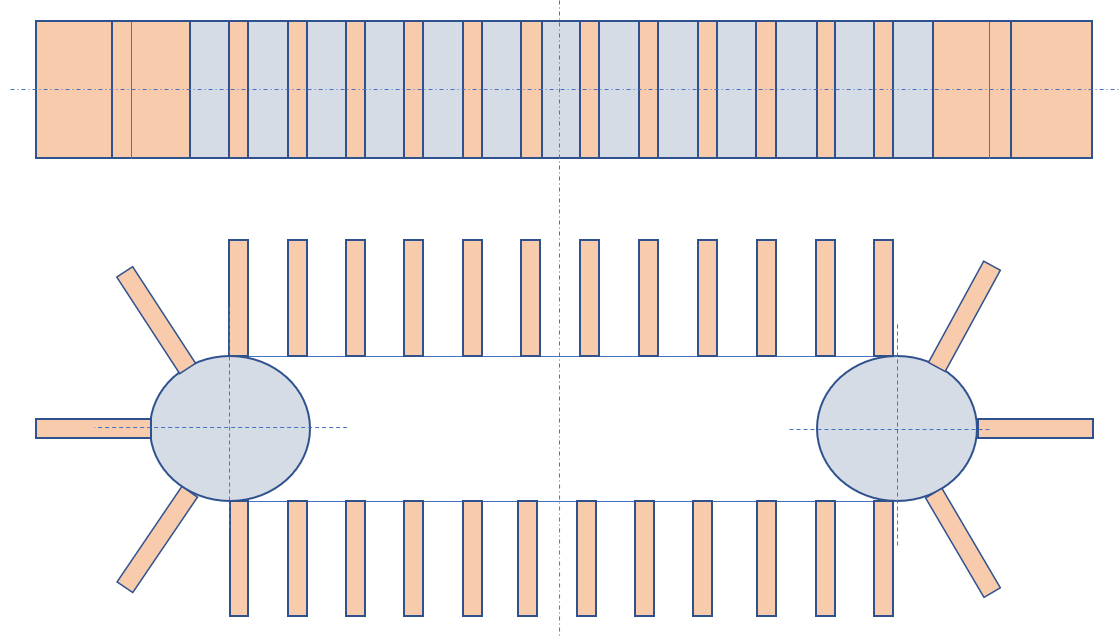
\includegraphics[width=0.30\textwidth]{Bilder/Powerpoint/Futtermagazin_horizontal}
  \end{center}
  \caption{Futtermagazin Horizontal}
  \label{Magazin Horizontal}
  \vspace{-10pt}
\end{wrapfigure} 

Das Futtermagazin Horizontal wäre für die erste Variante optimal. Da man den gewünschten Vorrat an Futterpackungen in die abgetrennten Räume platziert. Somit ist es einfach die gewünschte Position anzufahren und mit einen Greifer in die Schneideposition zu bringen. Der Aufbau ist wie ein Förderband, zwei Räder, ein Band mit oben platzierten Trennwänden und ein Motor der dieses Futtermagazin in Bewegung bringt. Zu beachten wäre wie die Futterpackungen ins Magazin eingelegt werden, nämlich mit der dünneren Fläche mit der Einkerbung die der Hersteller angegeben hat. Siehe Abbildung: \ref{Magazin Horizontal}

\subsubsection{Futtermagazin Vertikal}

\begin{wrapfigure}{r}{0.5\textwidth}
\vspace{-40pt}
  \begin{center}
    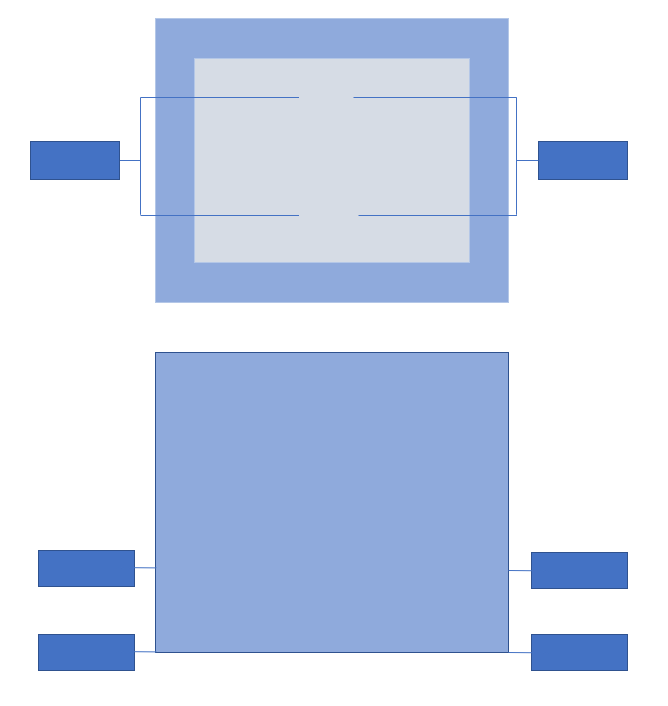
\includegraphics[width=0.3\textwidth]{Bilder/Powerpoint/Futtermagazin_vertikal}
  \end{center}
  \caption{Futtermagazin Vertikal}
  \label{Magazin Vertikal}
  \vspace{-10pt}
\end{wrapfigure}

Das Futtermagazin Vertikal ist ein rechteckiges Gehäuse an denen 4 Magnetzylinder platziert werden. In dieser Box kommen die 10 Futterpackungen. Der Ablauf funktioniert in einer gewissen Reihenfolge. Zuerst öffnet sich der erste linke Magnetzylinder danach der gegenüberliegende zweite Magnetzylinder. Daraufhin gelangt die erste Futterpackung auf die unteren Zylinder. Nach diesem Schritt schließen sich die beiden Magnetzylinder wieder, damit die anderen Packungen nach den öffnen der unteren Magnetzylinder nicht durch die Maschine fallen. Daraufhin wenn der Fütterungsbefehl kommt öffnen sich die unteren Zylinder und die Packung gleitet über ein Blech zur Schnittfläche. Der große Nachteil dieser Methode ist das immer wieder Fehler auftreten können. Die Futterpackung kann falsch an der Schneidfläche ankommen bzw. sich an einem bestimmten Ort verkeilen. Siehe Abbildung: \ref{Magazin Vertikal}


\section{Konstruktion der Wahlvariante und Details}

\subsection{Drehplatte}

\begin{wrapfigure}{r}{0.5\textwidth}
\vspace{-20pt}
  \begin{center}
    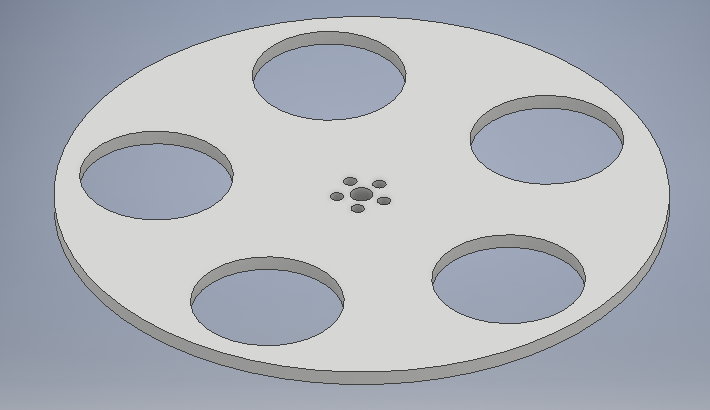
\includegraphics[width=0.30\textwidth]{Bilder/Inventor/Drehplatte}
  \end{center}
  \caption{Drehplatte Inventor}
  \label{Drehplatte_Inventor}
  \vspace{-10pt}
\end{wrapfigure}

Die Drehplatte besteht aus Aluminium und ist 10mm dick. Es werden 5 Löcher für die Schüsseln ausgeschnitten und in der Mitte ist ein Loch, in der eine Stahlwelle durch geht. Die Stahlwelle wurde deshalb ausgewählt, da sie erstens stabiler ist und somit kleiner bzw. mit kleinerem Durchmesser gewählt werden kann. Zweitens ist der Vierkant der in den Motor geht 4x4x20, dies ist für Aluminium sehr schmal da große Kräfte auftreten können und der Stift abreißen kann. Die Drehplatte wird auf der Welle mit einem Flansch befestigt damit das vertuschen nach oben, unten und zur Seite gesichert ist. Siehe Abbildung: \ref{Drehplatte_Inventor} \\

\begin{wrapfigure}{r}{0.5\textwidth}
\vspace{-20pt}
  \begin{center}
    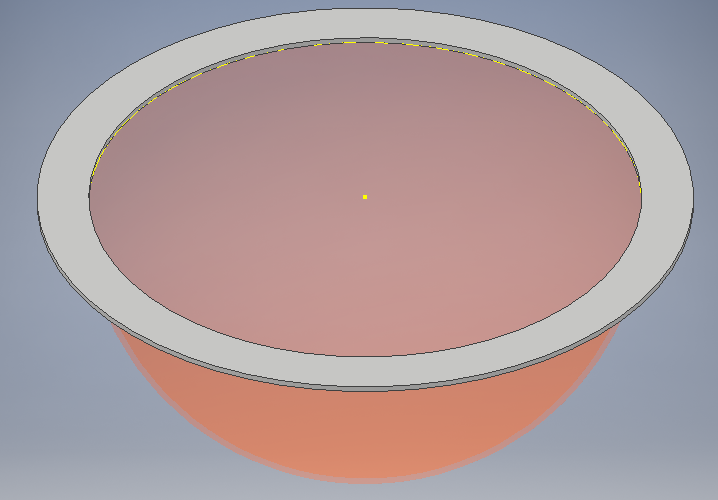
\includegraphics[width=0.26\textwidth]{Bilder/Inventor/Schuessel}
  \end{center}
  \caption{Futterschüssel Inventor}
  \label{Futterschuessel_Inventor}
  \vspace{-40pt}
\end{wrapfigure}

Die Futterschüssel hat deshalb einen Rand damit sie in ein Loch gelegt werden kann ohne dass sie durchfliegt, dennoch lässt sie sich leicht raus nehmen und reinigen. Durch eine rutschfeste Unterlage verrutsch die Schüssel nicht, auch wenn die Katze daraus frisst und sie mit Kraft die Schüssel zu verschieben versucht. Siehe Abbildung: \ref{Futterschuessel_Inventor}.

\subsection{Förderband, Kettenglied und Kettenrad}

\begin{figure}[H]
\begin{center}
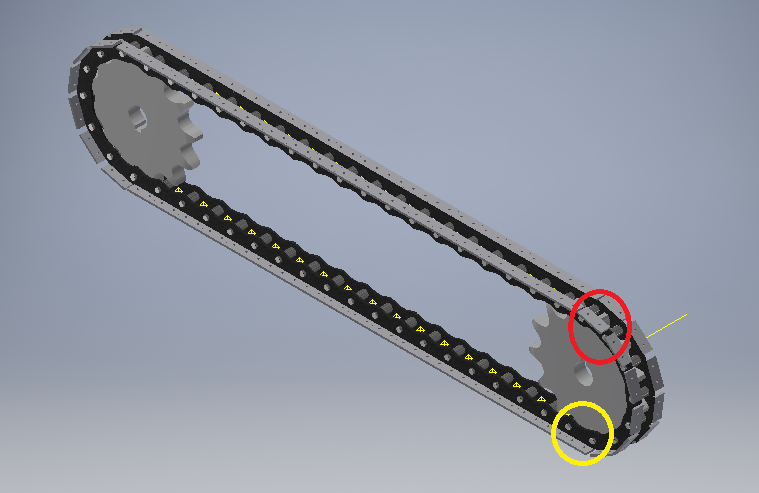
\includegraphics[width=10cm]{Bilder/Inventor/Kette}
\caption{Kette Inventor}
\label{Kette_Inventor} 
\end{center}
\end{figure}


Das Förderband Abbildung: \ref{Kette_Inventor} wurde in folgenden Schritten konstruiert: 

\begin{itemize}
\item[1] Als erstes wurde die Sicht in Inventor nach Vorne gedreht um die Grundlage des Förderbandes zu zeichnen.
\item[2] Zweitens wurde die Ebene YZ sichtbar gemacht und eine Ebene mit Versatz erstellt, die 234,95mm entfernt ist. In diesen beiden Ebenen kommen später die Kettenräder.
\item[3] Drittens wird auf der XY Ebene einen Kreis mit einen Durchmesser von 53,068mm gezeichnet. Der zweite Kreis in der gleiche Größe wird auf der erstellten Ebene platziert(234,95mm von der ersten Ebene entfernt). 
\item[4] Viertens werden die beiden Kreise an den obersten und untersten Punkten verbunden. Siehe gelber und roter Kreis.
\item[5] Fünftens wird an den beiden untersten Positionen der Kreise ein Punkt platziert. In Inventor existiert eine Methode namens Muster. Diese Funktion wird auf den Punkten platziert und die Richtung des Pfeiles nach rechts gedreht. Nun wird die Anzahl der Kettenglieder angegeben in unseren Fall 50. Die werden gleichmäßig über die Skizze verteilt.
\item[6] Sechstens wird eine neue Datei erstellt und das Kettenrad aus dem Inhaltscenter platziert. Siehe Abbildung \ref{Kettenrad_Inventor}.
\item[7] Siebtens wird das Kettenglied konstruiert und alle 3 Komponenten in ein gemeinsames Projekt eingefügt. Siehe Abbildung: \ref{Kettenglied_Inventor}.
\item[8] Achtens wird das Kettenglied am untersten Punkt des rechten Kreises abhängig gemacht.
\item[9] Neuntens Durch kann durch die Funktion Muster das Kettenglied gleichmäßig auf der Zeichnung platziert werden und dadurch entsteht die fertige Kette.
\item[10] Zehntens werden die Kettenräder auf den zuvor erstellten Ebenen abhängige gemacht. Danach ist die Kette fertig erstellt.\\
\end{itemize}

Das Kettenglied ist im Handel erhältlich. Die Anfertigung hat auf der Seite einen rechten Winkel auf denen Aluminiumplatten platziert sind. Auf diese Aluminiumplatten wird der Futterbeutel platziert. Siehe Abbildung: \ref{Kettenglied_Inventor}.\\

Das Kettenrad wurde aus dem Inhaltscenter platziert. Danach wurde eine Skizze angelegt und das Loch in der die Welle durch geht gezeichnet. Die Rundung für die Passfeder wurde darauf hin auch konstruiert damit das Kettenrad nicht auf der Welle durchrutscht und das Drehmoment übertragen kann. Siehe Abbildung: \ref{Kettenrad_Inventor}.

\begin{figure}[H]
   \begin{minipage}[hbt]{.4\linewidth} % [b] => Ausrichtung an \caption
      \includegraphics[width=\linewidth]{Bilder/Inventor/Kettenglied}
      \caption{Kettenglied Inventor}
      \label{Kettenglied_Inventor} 
   \end{minipage}
   \hspace{.2\linewidth}% Abstand zwischen Bilder
   \begin{minipage}[hbt]{.4\linewidth} % [b] => Ausrichtung an \caption
      \includegraphics[width=\linewidth]{Bilder/Inventor/Kettenrad}
      \caption{Kettenrad Inventor}
      \label{Kettenrad_Inventor}
   \end{minipage}
\end{figure}

\newpage
\subsection{Walze}

\begin{wrapfigure}{r}{0.5\textwidth}
\vspace{-20pt}
  \begin{center}
    \includegraphics[width=0.26\textwidth]{Bilder/Inventor/Rolle}
  \end{center}
  \caption{Walze Inventor}
  \label{Walze_Inventor}
  \vspace{-20pt}
\end{wrapfigure}

Die beiden Walzen sind aus Kunststoff innen hohl. Diese sind auch nicht auf der Welle befestigt sondern können sich frei drehen. Es ist nur auf jeder Seite ein Sicherungsring damit die beiden Walzen ihre Postion nicht verlassen.Siehe Abbildung: \ref{Walze_Inventor}. \\

\vspace{60pt}

\begin{wrapfigure}{r}{0.5\textwidth}
\vspace{-20pt}
  \begin{center}
    \includegraphics[width=0.26\textwidth]{Bilder/Inventor/Feder}
  \end{center}
  \caption{Feder Inventor}
  \label{Feder_Inventor}
\end{wrapfigure}

Die Feder drückt die beiden Walzen aneinander um die Futterpackung die durchgezogen wird auszuquetschen. Ohne die Feder und Walze könnte zu viele Reste in der Packung bleiben und so das ganze Futter verschwenden. Die Feder wurde von uns konstruiert und auf eine eigne Konstruktion gehängt die unabhängig von der Welle ist, damit die Feder nicht mitgedreht wird, sondern fix an einem Platz ist an den sie ihre Arbeit verrichtet. Siehe Abbildung: \ref{Feder_Inventor}.
\subsection{Hebelklemme}

\begin{wrapfigure}{r}{0.5\textwidth}
\vspace{-20pt}
  \begin{center}
    \includegraphics[width=0.40\textwidth]{Bilder/Inventor/Hebel_Klemme}
  \end{center}
  \caption{Hebelklemme Inventor}
  \label{Hebel_Klemme_Inventor}
  \vspace{-10pt}
\end{wrapfigure}

Die Hebelklemme dient zum Optimalen klemmen der Verpackung.
Es ähnelt einen Marmeladen Verschluss von früher. Die Packung wird zwischen den zwei Platte eingelegt, danach wird der Schließmechanismus auf der oberen Platte eingehakt, siehe roter Kreis. Daraufhin wird die Unterseite des Schließmechanismus nach unten gedrückt, siehe blauer Kreis.
Der Hebel wird soweit nach unten gedrückt bis er beim Stopper auftrifft, siehe gelber Kreis. Der Stopper hat die Aufgabe, dass der Hebel nicht zu weit geschlossen werden kann. Das hat zufolge das die Klemme leichter aufspringt. Siehe Abbildung: \ref{Hebel_Klemme_Inventor}.

\section{Berechnung und Dimensionierung}
\section{Simulation}	
\section{Bedienung und Wartung}

Bei der Entwicklung der Maschine wurde darauf geachtet, es Benutzerfreundlich als nur möglich zu gestalten. Darum lässt sich das Gehäuse der Maschine bis zur Hälfte Aufklappen um den Benutzer einen leichten Zugang zu verschaffen. Es mussten auch keine speziellen Vorkehrungen getroffen werden um den Benutzer zu schützen da es keine gefährlichen Stellen in der Maschine befinden die Personen schaden bzw. verletzen könnten. Die Befestigung der Futterpackungen ist auch ein leichtes durch den großen Platz der zur Verfügung steht und wenn man sich an folgende Schritte hält: 

\begin{itemize}
\item[1] Einspannen der Hinterseite der Packungen auf die Aluminiumplatten des Förderbandes. 
\item[2] Die Hebelklemme kurz nach der vom Futterhersteller vorgeschriebenen Schneidelinie festklemmen. (Dabei zu beachten, dass der Hebel in Richtung der Walze auf der rechten Seite befindet).
\item[3] Mit einer Schere oder Messer die Schneidelinie durchtrennen und den Abfall entsorgen.
\item[4] Die gewünschte Anzahl an Packungen festhängen, maximal 10 Packungen.
\end{itemize} 

Weiter zu Wartung, nachdem der Benutzer aus dem Urlaub zurück ist sollte man folgenden Teile der Maschine reinigen: 

\begin{itemize}
\item[1] Die Walze, hierbei kann durch das Ausquetschen der Packungen etwas Gelee an den beiden Walzen hängen bleiben. Einfach mit einem nassen Tuch diese abwischen.
\item[2] Die Futterschüsseln, diese können mit der Hand entnommen werden indem man auf der Unterseite der Platte die Schüssel nach oben drückt und mit der freien Hand die nimmt. Danach die Schüssel waschen und in die Platte zurück legen.
\item[3] Die Futterplatte, mit einem nassen Tuch die Oberfläche nach dem entfernen der Schüsseln reinigen.
\end{itemize}


\section{Selbstkritische Analyse und Ausblick}

Das Hauptproblem von meiner konstruierten Variante war das dichthalten der Packung mit einer Klemme die automatisch wenn das Förderband in betrieb ist leicht zu öffnen geht. Darum wurde die von uns konstruierte Hebel Klemme genommen. Die beim Betrieb des Förderbandes mit dem Hebel in eine Vorrichtung einhakt und diese dann die Klemme öffnet. \\
\\
Für Nachfolgeprojekte wäre besonders darauf zu achten das die Maschine von automatische gereinigt wird und womöglich eine Schneidefunktion einbauen die den Benutzer mehr entlasten könnte.\\
\\
Wenn ich in Zukunft noch einmal eine Katzenfuttermaschine bauen würde, würde ich diese nicht aus Packungen, sondern aus den kleinen Metallfutterpackungen mit der Lasche als Deckel. Der Benutzer müsste dann nur die Laschen so weit nach oben biegen damit der Deckel nicht aufgeht und in das Magazin einlegen. Die Packung wird daraufhin in Bewegung gebracht und die Lasche durch einen Haken geleitet. Dann öffnet sich die Packung und die Katze kann daraus fressen. Hat den Vorteil immer eine frische Schüssel zu haben und es können theoretisch so viele Packungen wie der Benutzer will in die Maschine eingelegt werden. \\
 
